\section{Computational Methodology}

\subsection{Lattice Boltzmann Method and Solver Formulation}
Unlike the Finite Volume Method (FVM), which discretizes the macroscopic Navier-Stokes equations and requires computationally expensive procedures to resolve pressure-velocity coupling, the Lattice Boltzmann Method (LBM) operates at the mesoscopic scale.
It solves the discrete Boltzmann transport equation, recovering macroscopic hydrodynamics via the Chapman-Enskog expansion \cite{chen1998lattice}.
This kinetic approach offers explicit time integration, exact linear advection, and local collision rules, making it highly efficient for handling the complex boundaries inherent to porous media.
The choice of LBM is particularly advantageous for the multi-physics problem addressed in this work, which couples viscous fingering, diffuse-interface phase-field thermodynamics, magnetostatic body forces, and Darcy--Brinkman resistance into a single simulation.
Four properties of the method are decisive in this context.
\emph{First}, the explicit two-step structure (local collision followed by linear streaming) keeps every operator local in space and avoids the global pressure-Poisson solve that dominates the runtime of incompressible Navier--Stokes codes;
this is essential because each simulation traverses thousands of LBM steps with $N_{sub} \in [5,20]$ nested Cahn--Hilliard substeps, so a global linear solve per step would be prohibitive.
\emph{Second}, body forces of any nature --- capillary, magnetic, or matrix drag --- can be injected through the Guo source term \cite{guo2002discrete} without altering the kernel itself;
the Chapman--Enskog analysis of Section~\ref{sec:chapman-enskog} proves that the discrete scheme recovers the target macroscopic momentum equation to $\mathcal{O}(\Delta t^{2})$ for arbitrary combinations of these forces.
\emph{Third}, the inclusion of the porous matrix is achieved at the level of the body force rather than through explicit obstacle geometry, so the same kernel transparently handles the free-flow ($K \to \infty$), Brinkman, and Darcy regimes as continuous limits of a single parameter, eliminating the ill-conditioned obstacle-resolution constraint that plagues pore-scale FVM simulations of low-permeability media.
\emph{Fourth}, the embarrassingly parallel structure of collision and streaming maps naturally onto Numba-compiled \texttt{@njit(parallel=True)} loops over $y$-rows, producing throughput sufficient to span the full $(\sigma, \chi_{\max}, K_0, m)$ parameter space required by the linear-stability analysis presented in the linear stability analysis chapter.
The spatial domain is discretized into a uniform global Cartesian mesh.
The velocity space at each node is quantized using the D2Q9 lattice model, which defines nine discrete velocity vectors $\mathbf{c}_i$: one rest particle, four cardinal, and four diagonal directions \cite{qian1992lattice}.
This specific lattice, illustrated in Figure~\ref{fig:d2q9-lattice}, provides the necessary symmetry and isotropy to correctly recover the full Navier-Stokes stress tensor in two dimensions.

\begin{figure}[H]
    \centering
    \framebox{\parbox{0.85\textwidth}{\centering
        \vspace{1.5cm}
        \textbf{[FIGURE TO CREATE: D2Q9 velocity lattice]}\\[10pt]
        \begin{minipage}{0.82\textwidth}\small\itshape
        Schematic of the D2Q9 velocity set centred on a single lattice node.
        Draw the nine discrete velocities $\bm{c}_i$ as arrows emanating from a central node: one rest particle ($i=0$, weight $w_0 = 4/9$, depicted as a filled dot at the origin), four cardinal vectors of length~$1$ ($i = 1,\ldots,4$, weights $w_i = 1/9$), and four diagonal vectors of length~$\sqrt{2}$ ($i = 5,\ldots,8$, weights $w_i = 1/36$).
        Label each arrow with its index $i$ and its weight $w_i$.
        Indicate the lattice spacing $\Delta x$ between nearest neighbours.
        Include a small auxiliary table (or legend) mapping every index to its canonical direction, e.g.\ $\bm{c}_1 = (+1, 0)$, $\bm{c}_2 = (0, +1)$, $\bm{c}_5 = (+1, +1)$, etc., to be cross-referenced by the Zou--He boundary diagram of Fig.~\ref{fig:zou-he-bc}.
        \end{minipage}
        \vspace{1.5cm}
    }}
    \caption{The D2Q9 velocity model used by the lattice Boltzmann kernel: nine discrete velocities $\bm{c}_i$ with associated weights $w_i$ on the uniform square lattice. The same indexing convention is used throughout this chapter for the description of the collision, streaming, and boundary-condition operators.}
    \label{fig:d2q9-lattice}
\end{figure}

The evolution of the system is governed by the discrete Lattice Boltzmann equation employing the single-relaxation-time Bhatnagar-Gross-Krook (BGK) collision operator \cite{bhatnagar1954model}.
To accurately couple the phase-field model and introduce macroscopic forces into the mesoscopic distributions, an exact forcing term $S_i$ \cite{guo2002discrete} is utilized:
\begin{equation}
    f_i(\mathbf{x} + \mathbf{c}_i \Delta t, t + \Delta t) = f_i(\mathbf{x}, t) - \frac{1}{\tau(\phi)} \left[ f_i(\mathbf{x}, t) - f_i^{eq}(\mathbf{x}, t) \right] + S_i \Delta t
\end{equation}
where $f_i$ are the density distribution functions, $\mathbf{c}_i$ are the discrete lattice velocities, and $\tau$ is the relaxation time.
The relaxation time $\tau(\phi)$ encodes the local kinematic viscosity through the standard Chapman--Enskog relation $\nu = c_s^{2}(\tau - 1/2)\,\Delta t$ derived in Section~\ref{sec:chapman-enskog}.
Because the two pure phases possess distinct viscosities $\nu_{\mathrm{inv}}$ and $\nu_{\mathrm{res}}$, the relaxation time must be evaluated locally from the phase fraction $S_{\mathrm{inv}} = (\phi+1)/2$.
Two interpolation rules are implemented in the kernel and selected at runtime through the boolean flag \texttt{VISC\_LINEAR}.
The first option computes a linear (arithmetic) average of the kinematic viscosities,
\begin{equation}
\nu_{\mathrm{eff}}^{\mathrm{lin}}(\phi)
\;=\; S_{\mathrm{inv}}\,\nu_{\mathrm{inv}}
\;+\; (1 - S_{\mathrm{inv}})\,\nu_{\mathrm{res}},
\label{eq:nu-linear}
\end{equation}
and is used only as a low-cost diagnostic for low mobility-ratio cases ($\nu_{\mathrm{res}}/\nu_{\mathrm{inv}} \lesssim 5$).
The default choice, adopted throughout the production runs reported in this work, is the harmonic mean
\begin{equation}
\boxed{\;\frac{1}{\nu_{\mathrm{eff}}(\phi)}
\;=\; \frac{S_{\mathrm{inv}}}{\nu_{\mathrm{inv}}}
\;+\; \frac{1 - S_{\mathrm{inv}}}{\nu_{\mathrm{res}}}.\;}
\label{eq:nu-harmonic}
\end{equation}
The reason for preferring~\eqref{eq:nu-harmonic} is physical, not algorithmic.
Across a sharp interface between two Newtonian fluids, the requirement of mechanical equilibrium imposes continuity of the tangential component of the viscous stress $\tau_{xy} = \nu\,\rho\,\partial_y u_x$, which in turn requires that the strain rate jumps inversely as the viscosity.
An arithmetic average~\eqref{eq:nu-linear} interpolates linearly the wrong quantity (the viscosity itself rather than its reciprocal) and consequently produces a smeared viscous-stress profile that fails the jump condition by a factor of order $\nu_{\mathrm{res}}/\nu_{\mathrm{inv}}$.
This generates spurious tangential body forces of the same order along the diffuse interface --- the well-known ``parasitic currents'' of diffuse-interface methods --- which would directly contaminate the LSA growth rate.
The harmonic mean~\eqref{eq:nu-harmonic} restores the jump condition to leading order in $\Delta x/W$ and is the standard choice in the multiphase LBM literature for ratios $\nu_{\mathrm{res}}/\nu_{\mathrm{inv}} \gg 1$ \cite{huang2015multiphaseLBM}.
The relaxation time recovered from~\eqref{eq:nu-harmonic} is $\tau(\phi) = 3\,\nu_{\mathrm{eff}}(\phi) + 1/2$, exactly as implemented in \texttt{lbm.py:62--65}.
The recovery of the \emph{multiphase porous} momentum equation by this scheme is not a postulate but a derived property: by injecting into $S_i$ a total force that simultaneously contains the diffuse-interface Korteweg stress $\bm{F}_c = \mu_c \nabla \phi$, the Kelvin magnetic body force $\bm{F}_m = -\tfrac{1}{2}|\bm{H}|^{2}\nabla\chi$, and a phase-weighted Darcy--Brinkman drag $\bm{F}_d = -\rho\,\uph/(K\lambda_{\mathrm{tot}})$ with two-phase mobility $\lambda_{\mathrm{tot}} = k_r^{\mathrm{inv}}/\nu_{\mathrm{in}} + k_r^{\mathrm{res}}/\nu_{\mathrm{out}}$, the Chapman--Enskog multiscale expansion (Section~\ref{sec:chapman-enskog}, equation~\eqref{eq:ce-final-mom}) yields exactly the generalised momentum balance
\begin{equation*}
\rho\bigl(\partial_t \uph + \uph\!\cdot\!\nabla\uph\bigr) = -\nabla P + \mu(\phi)\,\nabla^{2}\uph + \mu_c\,\nabla\phi - \tfrac{1}{2}|\bm{H}|^{2}\nabla\chi - \frac{\rho}{K\,\lambda_{\mathrm{tot}}}\,\uph,
\end{equation*}
i.e.\ the two-phase Darcy--Brinkman--Navier--Stokes--Kelvin equation.
The free-flow limit ($K\to\infty$), the single-phase Brinkman limit ($\phi \equiv \pm 1$), and the non-magnetic Saffman--Taylor limit ($\bm{H}_0 = \bm{0}$) all emerge as continuous parameter limits of the same kernel, without any change to the underlying algorithm.

\subsection{Cahn-Hilliard Solver: Spatial Discretization and Temporal Substepping}

The order parameter $\phi$ whose theoretical formulation was established in the Phase-Field Modeling section is evolved by a dedicated finite-difference module that runs alongside the LBM hydrodynamic kernel.
Because the advective Cahn-Hilliard equation
\begin{equation}
    \frac{\partial \phi}{\partial t} + \mathbf{u} \cdot \nabla \phi = M\,\nabla^2 \mu_c, \qquad \mu_c = 4\beta\,\phi(\phi^2 - 1) - \kappa\,\nabla^2 \phi,
\end{equation}
is fourth-order in $\phi$, a one-shot discretization would require a wide biharmonic stencil.
Instead, the implementation splits the update into two coupled second-order passes --- first computing the chemical potential field $\mu_c$ over the entire domain, then advancing $\phi$ using $\nabla^2 \mu_c$ --- which reduces every stencil to five points and makes the algorithm naturally local.

\subsubsection{Five-Point Isotropic Stencil}
All spatial derivatives are evaluated on the same uniform Cartesian grid used by the LBM kernel, with lattice spacing $\Delta x = 1$ in lattice units.
The Laplacian of any scalar field $\psi$ is approximated by the standard five-point stencil:
\begin{equation}
    \nabla^2 \psi(y, x) \approx \psi(y, x{+}1) + \psi(y, x{-}1) + \psi(y{+}1, x) + \psi(y{-}1, x) - 4\,\psi(y, x).
\end{equation}
The first spatial derivatives entering the advective term $\mathbf{u} \cdot \nabla \phi$ are computed using second-order centred differences, e.g.\ $\partial_x \phi \approx [\phi(y, x{+}1) - \phi(y, x{-}1)]/2$.

\begin{figure}[H]
    \centering
    \framebox{\parbox{0.88\textwidth}{\centering
        \vspace{1.5cm}
        \textbf{[FIGURE TO CREATE: Five-point Laplacian stencil and double-buffer update pattern]}\\[10pt]
        \begin{minipage}{0.85\textwidth}\small\itshape
        Two-panel figure.
        \textbf{Left panel --- Five-point isotropic stencil.}
        Draw a $3{\times}3$ block of grid nodes around a central point $(y, x)$.
        The central node is a filled circle labelled with coefficient $-4$; the four nearest neighbours $(y, x{\pm}1)$ and $(y{\pm}1, x)$ are open circles, each labelled with coefficient $+1$.
        The four corner nodes (diagonals) are absent from the stencil and may be drawn as faint dotted circles for contrast.
        Indicate the lattice spacing $\Delta x = 1$ between adjacent nodes.
        \textbf{Right panel --- Double-buffer update pattern.}
        Show two grid copies side by side, labelled \texttt{phi\_in} (representing $\phi^n$) and \texttt{phi\_out} (representing $\phi^{n+1}$).
        Use a five-point stencil overlay on \texttt{phi\_in} (the read pattern) and a single highlighted cell on \texttt{phi\_out} (the write target).
        A directed arrow from the read region to the write cell illustrates that the Euler update at each node consumes only $\phi^n$ values.
        A curved loop arrow between the two buffers (annotated ``swap'') indicates the pointer exchange performed externally between substeps.
        \end{minipage}
        \vspace{1.5cm}
    }}
    \caption{(Left) Five-point isotropic stencil used by the Cahn--Hilliard finite-difference module to evaluate Laplacians on the uniform Cartesian grid. (Right) Double-buffer update pattern: each substep reads only from \texttt{phi\_in} and writes only to \texttt{phi\_out}, the pointers being swapped externally between substeps to avoid in-place memory hazards.}
    \label{fig:five-point-and-buffer}
\end{figure}

The stencil depicted in Figure~\ref{fig:five-point-and-buffer} (left) carries a small leading-order anisotropy, but this is acceptable here because the Cahn-Hilliard relaxation acts on a thermodynamic timescale much shorter than the hydrodynamic timescale, smoothing out grid-induced artefacts.
By contrast, the macroscopic force computation in the LBM kernel uses the more demanding 9-point isotropic stencil, since spurious anisotropic currents at the interface would directly contaminate the momentum balance.

\subsubsection{Boundary Conditions}
The boundary treatment of the order parameter is fully consistent with the boundary conditions imposed by the LBM kernel.
The transverse boundaries ($y = 0$ and $y = N_y - 1$) are always treated as periodic, mirroring the spanwise periodicity of the LBM mesh.
The longitudinal boundaries depend on the simulation mode:
\begin{itemize}
    \item \textbf{Inlet ($x = 0$, injection mode):} a Dirichlet condition $\phi = +1$ is enforced, representing the continuous injection of the pure invading phase.
    The condition is reapplied both before computing $\mu_c$ and after the temporal update, to prevent the explicit Euler step from disturbing the boundary value through the centred-difference advective stencil.
    \item \textbf{Outlet ($x = N_x - 1$):} a homogeneous Neumann condition $\partial_x \phi = 0$ is enforced by copying the value from the adjacent internal node, $\phi_{N_x-1} = \phi_{N_x-2}$.
    This allows the interface to be advected smoothly out of the computational domain without spurious reflection.
    \item \textbf{Chemical potential $\mu_c$ at both $x$-boundaries:} homogeneous Neumann ($\partial_x \mu_c = 0$).
    Physically, this nullifies the diffusive flux $M \nabla \mu_c$ across the longitudinal boundaries --- at the inlet, the phase composition is dictated by the injection Dirichlet condition, not by diffusion;
    at the outlet, the only allowed mass flux is the advective sweep by the velocity field.
\end{itemize}
For fully periodic configurations (e.g.\ spatially periodic linear-stability test cases), both $x$-boundaries are treated periodically through modular indexing, identical to the $y$ treatment.

\subsubsection{Explicit Euler Update and Numerical Safeguards}\label{sec:cahnhilliard-update}
After the chemical potential field has been finalised, the order parameter is advanced through an explicit first-order Euler scheme:
\begin{equation}
    \phi^{n+1}(y, x) = \phi^n(y, x) + \Delta t_{CH}\left[ M\,\nabla^2 \mu_c - \left(u_x\,\partial_x \phi + u_y\,\partial_y \phi\right) \right].
\end{equation}
The velocity field $(u_x, u_y)$ here is the physical velocity recovered from the Guo forcing scheme described below.
To prevent unphysical overshoots of the order parameter beyond the bulk equilibrium values $\phi = \pm 1$ --- overshoots that the quartic bulk term of $\mathcal{F}$ can amplify into catastrophic numerical blow-up --- the updated values are clamped to the physical interval $\phi^{n+1} \in [-1, +1]$ before being stored.
In well-resolved simulations (sufficient interface thickness and properly calibrated mobility), the clamp is essentially never active and the associated mass error is negligible;
the clamp is retained as a numerical safety net for transient instabilities, e.g.\ during the start-up phase or near very high mobility-ratio interfaces.
The update is implemented through the double-buffer pattern of Figure~\ref{fig:five-point-and-buffer} (right) so that the right-hand side at each grid point is evaluated using the field $\phi^n$ everywhere, never with partially updated values from earlier in the sweep.
The buffer pointers are swapped externally between substeps, avoiding any in-place memory hazard.

\subsubsection{Temporal Substepping and the Biharmonic CFL Constraint via Von Neumann Analysis}

Because the Cahn-Hilliard equation is fourth-order in space, the explicit Euler scheme adopted in the previous paragraph is subject to a far more restrictive stability bound than the convective CFL of the LBM kernel ($\Delta t_{LBM} \lesssim \Delta x / c_s$).
Rather than postulating this restriction empirically, we derive it from a rigorous Von Neumann (discrete Fourier) stability analysis applied to the stiffness-dominating fourth-derivative term.
The same calculation simultaneously identifies the most numerically dangerous wave mode, fixes the safety factor used in the code, and explains \emph{quantitatively} why the substepping ratio $N_{sub}$ must be chosen as it is.

\paragraph{Linearised model equation.} The advective Cahn-Hilliard equation contains three structurally distinct terms: the advection $\mathbf{u}\!\cdot\!\nabla\phi$, the non-linear chemical-potential reaction $4\beta\,\phi(\phi^2-1)$, and the biharmonic relaxation $-M\kappa\,\nabla^4\phi$.
The first two terms produce bounded contributions to the amplification factor: advection is convectively stable for any centred-difference Euler integrator provided $|\mathbf{u}|\,\Delta t/\Delta x \leq 1$ (the classical hyperbolic CFL), while the reaction term contributes an $\mathcal{O}(\Delta t)$ correction that is dominated by the biharmonic in the asymptotic regime $\Delta x \to 0$.
The genuinely \emph{stiff} contribution --- the one which forces the substepping --- is the fourth-derivative diffusion.
Isolating it in one spatial dimension yields the linearised model PDE
\begin{equation}
    \frac{\partial \phi}{\partial t} = -M\kappa\,\frac{\partial^4 \phi}{\partial x^4},
\end{equation}
which is itself the linearised image of $\partial_t\phi = M\,\nabla^2\mu_c$ around a uniform reference state, with $\mu_c \approx -\kappa\,\nabla^2\phi$ as the dominant contribution to the chemical potential at short wavelengths.

\paragraph{Spatial-temporal discretisation.} Applying explicit Euler in time and central finite differences in space, and composing the five-point Laplacian stencil with itself, the discrete biharmonic operator at node $j$ reads
\begin{equation}
    \left(\frac{\partial^4 \phi}{\partial x^4}\right)_j \approx \frac{1}{(\Delta x)^4}\left( \phi_{j+2}^n - 4\phi_{j+1}^n + 6\phi_j^n - 4\phi_{j-1}^n + \phi_{j-2}^n \right),
\end{equation}
so the explicit update at grid node $j$ and time level $n$ is
\begin{equation}
    \phi_j^{n+1} = \phi_j^n - \frac{M\kappa\,\Delta t}{(\Delta x)^4}\left( \phi_{j+2}^n - 4\phi_{j+1}^n + 6\phi_j^n - 4\phi_{j-1}^n + \phi_{j-2}^n \right).
\end{equation}
For algebraic compactness we introduce the dimensionless biharmonic Fourier number
\begin{equation}
    r \;\equiv\; \frac{M\,\kappa\,\Delta t}{(\Delta x)^4}.
\end{equation}

\paragraph{Insertion of the Fourier ansatz.} Following Von Neumann, we exploit the linearity of the scheme: any numerical error obeys the same recurrence as $\phi$ itself.
We decompose the error into a discrete Fourier series and analyse a single harmonic mode of spatial wavenumber $k$,
\begin{equation}
    \epsilon_j^n = E^n\,e^{i\,k\,x_j}, \qquad x_j = j\,\Delta x,
\end{equation}
where $E^n$ is the (complex) amplitude at time level $n$ and $i = \sqrt{-1}$.
Substituting into the discrete update and dividing through by $E^n e^{ikx_j}$:
\begin{equation}
    G(k) \;\equiv\; \frac{E^{n+1}}{E^n} = 1 - r\left[\, e^{i\,2k\Delta x} - 4 e^{i\,k\Delta x} + 6 - 4 e^{-i\,k\Delta x} + e^{-i\,2k\Delta x}\,\right].
\end{equation}
Collecting conjugate pairs through Euler's identity $e^{i\theta} + e^{-i\theta} = 2\cos\theta$,
\begin{equation}
    G(k) = 1 - r\bigl[\,2\cos(2k\Delta x) - 8\cos(k\Delta x) + 6\,\bigr].
\end{equation}
The bracketed expression is precisely the spectral symbol of the discrete biharmonic operator.
Applying the half-angle identity $1 - \cos\theta = 2\sin^2(\theta/2)$ twice (once to each cosine) and using $\cos(2\theta) = 1 - 2\sin^2\theta$,
\begin{align}
    2\cos(2k\Delta x) - 8\cos(k\Delta x) + 6
    &= 2\bigl[1 - 2\sin^2(k\Delta x)\bigr] - 8\cos(k\Delta x) + 6 \nonumber \\
    &= 8 - 4\sin^2(k\Delta x) - 8\cos(k\Delta x) \nonumber \\
    &= 8\bigl[1 - \cos(k\Delta x)\bigr] - 4\sin^2(k\Delta x) \nonumber \\
    &= 16\sin^2(k\Delta x/2) - 16\sin^2(k\Delta x/2)\cos^2(k\Delta x/2) \nonumber \\
    &= 16\sin^4(k\Delta x/2).
\end{align}
We thus arrive at the compact closed-form amplification factor of the explicit biharmonic stencil:
\begin{equation}
    \boxed{\;G(k) = 1 - 16\,r\,\sin^4\!\!\left(\frac{k\,\Delta x}{2}\right)\;}
\end{equation}

\paragraph{Stability condition.} The Lax-Richtmyer equivalence theorem requires that, for the consistent scheme to converge, no Fourier mode may be amplified, i.e.\ $|G(k)| \leq 1$ for every admissible wavenumber $k$. Since $r > 0$ and $\sin^4(\cdot)$ is non-negative, $G(k) \leq 1$ trivially.
The non-trivial inequality is $G(k) \geq -1$:
\begin{equation}
    16\,r\,\sin^4\!\!\left(\frac{k\,\Delta x}{2}\right) \leq 2.
\end{equation}
The discrete grid admits wavenumbers in the Nyquist-limited range $k\Delta x \in [0, \pi]$.
The amplification is monotonic in $\sin^4(k\Delta x/2)$ and therefore extremised at the highest representable wavenumber, the \emph{Nyquist mode} $k\Delta x = \pi$ (wavelength $\lambda = 2\Delta x$, the saw-tooth oscillation between adjacent grid points), where $\sin^4(\pi/2) = 1$.
Imposing the bound on this worst-case mode:
\begin{equation}
    16\,r \leq 2 \;\Longleftrightarrow\; r \leq \tfrac{1}{8}.
\end{equation}
Returning to dimensional variables, the absolute one-dimensional stability bound of the explicit biharmonic stencil reads
\begin{equation}
    \boxed{\;\Delta t_{CH} \leq \frac{(\Delta x)^4}{8\,M\,\kappa} \quad \text{(1D)}\;}
\end{equation}
The behaviour of $G(k)$ across the three regimes (stable, marginal, and unstable) is summarised in Figure~\ref{fig:vn-stability}, which makes graphically apparent why the bound is saturated by the Nyquist mode and why even moderate over-estimates of $r$ lead to geometric divergence.

\begin{figure}[H]
    \centering
    \framebox{\parbox{0.88\textwidth}{\centering
        \vspace{1.5cm}
        \textbf{[FIGURE TO CREATE: Amplification factor $G(k)$ vs.\ wavenumber]}\\[10pt]
        \begin{minipage}{0.85\textwidth}\small\itshape
        Plot of the discrete amplification factor $G(k) = 1 - 16\,r\,\sin^4(k\Delta x/2)$ as a function of the dimensionless wavenumber $k\Delta x \in [0, \pi]$, for three representative values of the biharmonic Fourier number $r = M\kappa\,\Delta t/(\Delta x)^4$:
        \begin{itemize}\itemsep0pt
            \item $r = 1/16$ --- safely stable; $G(k)$ stays well inside the strip $|G| \le 1$.
            \item $r = 1/8$ --- marginally stable; $G(k)$ touches the lower bound $-1$ exactly at the Nyquist mode $k\Delta x = \pi$.
            \item $r \approx 0.16$ --- $\sim 25\%$ above the critical value; $G(k=\pi) \approx -1.5$, in the unstable region.
        \end{itemize}
        Shade the stability strip $|G| \le 1$ in light grey. Draw dashed horizontal lines at $G = \pm 1$ for visual reference, and a vertical dashed line at the Nyquist wavenumber $k\Delta x = \pi$. Annotate the critical bound $r = 1/8$ on the corresponding curve. Optionally include a small inset panel showing the geometric divergence $E^n = G^n E^0$ when $G < -1$, illustrating the alternating-sign checkerboard blow-up described in the text.
        \end{minipage}
        \vspace{1.5cm}
    }}
    \caption{Amplification factor $G(k) = 1 - 16\,r\,\sin^4(k\Delta x/2)$ of the explicit biharmonic stencil for three values of the dimensionless Fourier number $r = M\kappa\,\Delta t/(\Delta x)^4$. The worst-case Nyquist mode $k\Delta x = \pi$ saturates the bound and dictates the 1D stability limit $r \le 1/8$ derived in the text.}
    \label{fig:vn-stability}
\end{figure}

\paragraph{Extension to two dimensions.} In the isotropic 2D Cartesian implementation of the present work, the chemical potential field $\mu_c$ is itself constructed from a five-point Laplacian, and the divergence of the diffusive flux $M\,\nabla^2\mu_c$ folds a second five-point stencil on top.
The resulting compound operator contains pure derivatives $\partial^4_x$, $\partial^4_y$ \emph{and} mixed $\partial^2_x\partial^2_y$ contributions.
Applying the same Von Neumann ansatz $\epsilon = E\,e^{i(k_x x + k_y y)}$ to the 2D scheme yields the amplification factor
\begin{equation}
    G_{2D}(k_x, k_y) = 1 - 16\,r\left[\sin^4\!\!\left(\frac{k_x\Delta x}{2}\right) + \sin^4\!\!\left(\frac{k_y\Delta y}{2}\right) + 2\sin^2\!\!\left(\frac{k_x\Delta x}{2}\right)\sin^2\!\!\left(\frac{k_y\Delta y}{2}\right)\right].
\end{equation}
On an isotropic grid ($\Delta x = \Delta y$), the worst-case mode is the corner Nyquist $(k_x, k_y) = (\pi/\Delta x, \pi/\Delta x)$, for which each $\sin^4$ term equals unity and the mixed product also equals unity, so the bracket reaches its maximum value of $4$.
The stability condition $16r\cdot 4 \leq 2$ tightens the bound by a factor of four:
\begin{equation}
    \boxed{\;\Delta t_{CH} \leq \frac{(\Delta x)^4}{32\,M\,\kappa} \quad \text{(2D, isotropic)}\;}
\end{equation}
This factor-of-four tightening relative to the 1D estimate is precisely why a naive single-step Cahn-Hilliard update embedded inside the LBM cycle fails catastrophically for the parameter combinations used in this work --- and why the substepping strategy is not optional but structurally required.

\paragraph{Physical manifestation of the instability.} For a given $r$, suppose the bound is violated such that $G(\pi/\Delta x) = -1 - \delta$ with $\delta > 0$ (e.g.\ $G = -1.5$ when $r$ is approximately $25\%$ above the critical value).
The recurrence $E^{n+1} = G\,E^n$ then generates the sequence
\begin{equation}
    E^1 = -1.5\,E^0, \quad E^2 = +2.25\,E^0, \quad E^3 = -3.375\,E^0, \quad \ldots
\end{equation}
The two-fold signature of biharmonic instability is therefore unmistakable in practice: (i) the unstable mode is the shortest representable wavelength ($\lambda = 2\Delta x$), so the divergent signal manifests as a checkerboard pattern alternating between adjacent grid nodes;
and (ii) because $G < 0$, the amplitude oscillates in sign between successive time levels --- the field flips $\pm$ at each step while its magnitude grows geometrically.
Quartic over-shoots beyond $|\phi| > 1$ trigger the bulk term $4\beta\phi(\phi^2-1)$ in $\mu_c$ to invert direction (its derivative changes sign for $|\phi| > 1/\sqrt{3}$), at which point the thermodynamic restoring force becomes catastrophically destabilising.
The $\phi \in [-1,+1]$ clamp introduced in Sec.~\ref{sec:cahnhilliard-update} would then mask the blow-up locally but pollute the global mass balance;
the substepping is the principled cure that prevents the instability from being triggered in the first place.

\paragraph{Practical implementation in the code.} The runtime selection of $N_{sub}$ implements the 2D stability bound with a conservative safety margin.
Targeting $r_{eff} \equiv M\,\kappa\,\Delta t_{CH}/(\Delta x)^4 \leq 1/32 \times \mathcal{S}$ (with safety factor $\mathcal{S} \approx 0.8$, equivalent to operating at $80\%$ of the analytical limit), and recalling that $\Delta t_{CH} = \Delta t_{LBM}/N_{sub} = 1/N_{sub}$ in lattice units,
\begin{equation}
    N_{sub} \;\geq\; \left\lceil \frac{32\,M\,\kappa}{\mathcal{S}\,(\Delta x)^4} \right\rceil.
\end{equation}
For the simulations presented in this work --- where $\kappa$ scales linearly with $\sigma\,W$ through the calibration $\kappa = 3\sigma W/4$ and the mobility $M$ is fixed to balance the Péclet number of the interface --- this prescription yields typical values $N_{sub} \in [5, 20]$, with the upper end of the range required for high interfacial tension ($\sigma \to \sigma_{max}$) and/or thick interfaces ($W \to W_{max}$).
Larger $N_{sub}$ improves the conditioning of the explicit Euler integrator at the cost of a proportional increase in serial computational work per LBM step;
the trade-off is acceptable because each substep is itself trivially parallelised through Numba's \texttt{prange} and operates on the same compact five-point stencil, so the marginal cost of doubling $N_{sub}$ is essentially the bandwidth of two extra five-point sweeps per LBM iteration.

\subsubsection{Parallelization and Coupling}
The substep routine is compiled by Numba with \texttt{@njit(parallel=True, cache=True)}, and the outer loop over transverse rows ($y$) is parallelised using \texttt{prange}.
Because the five-point stencil is local and the temporal update writes only to \texttt{phi\_out}, there are no inter-row data dependencies and the parallel reduction is embarrassingly parallel.
The chemical-potential computation and the temporal update are kept in separate parallel passes because the second pass reads $\mu_c$ at the four nearest neighbours and therefore requires the $\mu_c field$ to be fully populated across all rows before any value of $\phi^{n+1}$ is computed.
This two-phase structure is the algorithmic image of the second-order operator splitting of the original fourth-order equation.
At the end of each LBM step, the updated phase field $\phi$ is consumed by three physically distinct couplings in the next iteration: the heterogeneous magnetic susceptibility $\chi(\phi)$ used by the Poisson solver, the local permeability $K(\phi)$ used by the Guo forcing scheme, and the interpolated kinematic viscosity $\nu(\phi)$ entering the BGK relaxation time.
The capillary body force $\mathbf{F}_s = \mu_c \nabla \phi$ is reassembled inside the LBM kernel from the latest $\phi$ field rather than being passed in from the Cahn-Hilliard module, so that all three macroscopic forces ($\mathbf{F}_s$, $\mathbf{F}_m$, and the Darcy drag) act on the same instantaneous phase configuration.

\subsection{External Forcing: Interfacial and Magnetic Couplings}
The total macroscopic body force $\mathbf{F} = \mathbf{F}_s + \mathbf{F}_m$ acts as a source term for the momentum update at each discrete time step.
The capillary force is recovered directly from the Cahn--Hilliard chemical potential, as derived in the Phase-Field Modeling section:
\begin{equation}
\bm{F}_c \;=\; \mu_c\,\nabla\phi
    \;=\; \bigl[4\beta\,\phi(\phi^{2} - 1) - \kappa\,\nabla^{2}\phi\bigr]\,\nabla\phi.
\label{eq:Fc-recall}
\end{equation}
The magnetic force, as derived rigorously in Section~\ref{sec:kelvin-heterogeneous}, is the divergence of the Maxwell stress tensor evaluated for a linear magnetisable medium with spatially varying susceptibility:
\begin{equation}
\bm{F}_m \;=\; -\,\tfrac{1}{2}\,|\bm{H}|^{2}\,\nabla\chi(\phi),
\qquad
\bm{H} \;=\; \bm{H}_0 \;-\; \nabla\tilde{\psi}.
\label{eq:Fm-recall}
\end{equation}
The total field $\bm{H}$ is reconstructed at each grid point by finite-differencing the perturbative potential $\tilde{\psi}$ delivered by the magnetostatic Poisson solver of Section~\ref{sec:poisson-solver-patch}.
All spatial derivatives entering \eqref{eq:Fc-recall} and \eqref{eq:Fm-recall} are evaluated with the standard five-point isotropic Laplacian
\begin{equation}
\nabla^{2}\psi(y, x) \;\approx\; \psi(y, x{+}1) + \psi(y, x{-}1) + \psi(y{+}1, x) + \psi(y{-}1, x) - 4\,\psi(y, x),
\end{equation}
and second-order centred differences for the gradients.
The five-point stencil carries a leading-order grid anisotropy of order $(\Delta x)^{2}|\partial^{4}\psi|$, which for the present problem is acceptable for three reasons.
First, the order parameter $\phi$ is already smoothed to a tanh profile of width $W \geq 4\,\Delta x$ inside the diffuse interface, where derivatives of fourth order remain bounded.
Second, the perturbative potential $\tilde{\psi}$ is harmonic in each pure phase (the source $\bm{H}_0\!\cdot\!\nabla\mu_r$ is supported only on the interface), so $|\partial^{4}\tilde{\psi}|$ is small away from the band where $\nabla\chi$ acts.
Third, the spurious anisotropy of a five-point stencil scales with the Laplacian itself, not with the gradient, and therefore does not enter the gradient-based force expressions to leading order.
A migration to a nine-point isotropic stencil --- which would reduce the anisotropy to fourth order in $\Delta x$ at the cost of $80\%$ more floating-point operations per node --- is reserved as a future-work improvement once the linear-stability validation is complete and parasitic-current diagnostics motivate it quantitatively.
The Kelvin body force adopted here belongs to the family of magnetostatic stresses derived from the Maxwell stress tensor $T_{ij}^{M} = \mu_0\,H_i H_j - \tfrac{1}{2}\mu_0|\bm{H}|^{2}\delta_{ij}$, whose divergence reduces, for a linear magnetisable medium with susceptibility $\chi(\bm{x})$ and in the absence of free currents, to $\bm{f}_m = -\tfrac{1}{2}\mu_0|\bm{H}|^{2}\nabla\chi$ \cite{rosensweig1985ferrohydrodynamics}.
This is the form adopted in the simulation framework of Gontijo and Cunha \cite{gontijo_cunha_review} for ferrofluid hydrodynamics in the linear-response regime, where the susceptibility is computed from a constitutive law (here $\chi(\phi) = \chi_{\max}(\phi+1)/2$) and the magnetic field itself is reconstructed from the scalar magnetic potential via $\bm{H} = \bm{H}_0 - \nabla\tilde{\psi}$, with $\tilde{\psi}$ obtained by solving the generalised Poisson equation $\divg[\mu_r(\phi)\nabla\tilde{\psi}] = \bm{H}_0\!\cdot\!\nabla\mu_r$.
The use of a scalar potential (as opposed to a direct integration of $\bm{H}$) is the same strategy employed in the references cited above: it reduces a vector boundary-value problem to a single scalar elliptic equation that can be solved by standard relaxation methods (Gauss--Seidel SOR in our implementation), and automatically enforces the constraint $\nabla\times\bm{H} = \bm{0}$ at the discrete level.

\begin{figure}[H]
    \centering
    \framebox{\parbox{0.92\textwidth}{\centering
        \vspace{1.5cm}
        \textbf{[FIGURE TO CREATE: Magnetic Force Discretization Scheme]}\\[10pt]
        \begin{minipage}{0.88\textwidth}\small\itshape
        Diagrama de blocos comparativo ilustrando as vantagens numéricas da formulação pelo potencial escalar magnetostático.
        \textbf{Painel Superior (Abordagem Tensorial Direta):} Sequência computacional $\bm{H} \rightarrow \nabla \bm{H} \rightarrow \nabla \cdot T_{ij}^M$. Adicionar uma anotação indicando que o cálculo numérico de derivadas de segunda ordem causa degradação do erro de truncamento para $\mathcal{O}(\Delta x)$ na interface e a perda de consistência variacional (gerando correntes espúrias tangenciais).
        \textbf{Painel Inferior (Abordagem Adotada - Potencial Escalar):} Sequência computacional $\tilde{\psi} \rightarrow \bm{H} \rightarrow |\bm{H}|^2 \rightarrow -\frac{1}{2}\mu_0|\bm{H}|^2\nabla\chi$. Adicionar uma anotação destacando que o uso exclusivo de gradientes de primeira ordem preserva a precisão $\mathcal{O}(\Delta x^2)$ do LBM e assegura a consistência variacional estrita com a minimização da energia magnetostática $\mathcal{E}[\tilde{\psi}]$.
        \end{minipage}
        \vspace{1.5cm}
    }}
    \caption{Fluxo esquemático da discretização da força magnética de Kelvin. A estratégia computacional via potencial escalar $\tilde{\psi}$ adotada neste solver garante a manutenção da ordem de precisão espacial do método Lattice Boltzmann e impõe consistência variacional, mitigando o surgimento de correntes espúrias e erros de anisotropia de malha na interface.}
    \label{fig:kelvin-discretization-scheme}
\end{figure}

\subsection{Darcy Resistance and Kinematic Recovery (Guo Scheme)}
\label{sec:darcy-drag-patch}

To represent the resistance imposed by the porous matrix without explicit obstacle geometry, the kernel implements the Guo forcing scheme of \cite{guo2002discrete} with a body-force contribution
\begin{equation}
\bm{F}_d \;=\; -\,\sigma_D(\phi, \bm{x})\,\rho\,\bm{u},
\qquad
\sigma_D \;\equiv\; \frac{1}{K(\bm{x})\,\lambda_{\mathrm{tot}}(\phi)},
\label{eq:Fd-twophase}
\end{equation}
where $K(\bm{x})$ is the local intrinsic permeability (a property of the rock matrix) and $\lambda_{\mathrm{tot}}(\phi)$ is the two-phase total kinematic mobility~\eqref{eq:lambda-tot} introduced in the Relative Permeability section.
The drag coefficient $\sigma_D$ has units of inverse time and reduces correctly to the textbook single-phase form $\nu/K$ when the medium is occupied by a single fluid ($\lambda_{\mathrm{tot}} = 1/\nu_\alpha$).
The drag force is velocity-dependent, which couples it implicitly to the very momentum it modifies.
Solving for the physical fluid velocity from the macroscopic moment relation $\rho\bm{u} = \sum_i f_i\bm{c}_i + (\Delta t/2)\bm{F}_{\mathrm{tot}}$, with $\bm{F}_{\mathrm{tot}} = \bm{F}_c + \bm{F}_m - \sigma_D\rho\bm{u}$, yields the closed-form inversion
\begin{equation}
\boxed{\; \bm{u}(\bm{x}, t)
\;=\; \frac{\bm{u}^{\star}}{1 + \tfrac{1}{2}\,\sigma_D},
\qquad
\bm{u}^{\star}
\;=\; \frac{1}{\rho}\!\left(\sum_i f_i\,\bm{c}_i
+ \tfrac{\Delta t}{2}(\bm{F}_c + \bm{F}_m)\right).
\;}
\label{eq:uphys-implicit}
\end{equation}
This is the operation performed at \texttt{lbm.py:84--85}.
The analytical inversion is essential when $\sigma_D\,\Delta t/2 \gtrsim 1$ (low-permeability regimes), because an explicit treatment would require $\sigma_D\,\Delta t < 2$ for stability --- a constraint that collapses the time step by orders of magnitude precisely in the parameter regime where viscous fingering is most aggressive.
The total force re-injected into the Guo source for the next collision is finally
\begin{equation}
\bm{F}_{\mathrm{tot}}(\bm{x}, t)
\;=\; \bm{F}_c(\bm{x}, t) + \bm{F}_m(\bm{x}, t) - \sigma_D\,\rho\,\bm{u}(\bm{x}, t),
\label{eq:Ftot-final}
\end{equation}
with $\bm{u}$ taken from~\eqref{eq:uphys-implicit}.
The free-flow regime is recovered as the continuous limit $K\to\infty$, in which $\sigma_D \to 0$, the denominator of \eqref{eq:uphys-implicit} collapses to unity, and the drag contribution to \eqref{eq:Ftot-final} vanishes identically.
The same kernel therefore transparently handles the free-fluid, Brinkman, and Darcy regimes as parameter limits of a single permeability field $K(\bm{x})$, without conditional branches or geometric obstacles --- the same observation that motivated the algorithmic choice in the opening overview of the LBM kernel.

\subsection{Magnetostatic Poisson Solver: Discretisation and Successive Over-Relaxation}
\label{sec:poisson-solver-patch}

The perturbative magnetostatic potential $\tilde{\psi}(\bm{x}, t)$ introduced in~\eqref{eq:helmholtz-decomp} is the solution of the heterogeneous generalised Poisson equation~\eqref{eq:poisson-psitilde}, restated here for convenience:
\begin{equation}
\nabla\!\cdot\!\bigl[\mu_r(\phi)\,\nabla\tilde{\psi}\bigr]
\;=\; \bm{H}_0\!\cdot\!\nabla\mu_r(\phi).
\label{eq:poisson-restated}
\end{equation}
This is an elliptic boundary-value problem whose non-locality forces a global linear solve at every coupling step.
Unlike the LBM and Cahn--Hilliard updates, which are purely local in space, the Poisson update is the only global operation in the algorithm and its cost governs the time-to-solution at the parameter regimes of interest.

\paragraph{Finite-volume discretisation.}
The equation is discretised on the same uniform Cartesian grid used by the LBM kernel ($\Delta x = \Delta y = 1$ in lattice units) using a cell-centred finite-volume scheme that integrates the conservative divergence form of~\eqref{eq:poisson-restated} over each control volume $\Omega_{ij}$:
\begin{equation}
\oint_{\partial\Omega_{ij}}\!\mu_r\,\nabla\tilde{\psi}\!\cdot\!\hat{\bm{n}}\,dS
\;=\; \int_{\Omega_{ij}}\!\bm{H}_0\!\cdot\!\nabla\mu_r\,d\Omega.
\label{eq:fv-integral}
\end{equation}
The surface integral on the left-hand side decomposes into four face fluxes (east, west, north, south).
The relative permeabilities at the cell faces are obtained by arithmetic averaging of the values at the two adjacent nodes,
\begin{equation}
\mu_E = 1 + \tfrac{1}{2}(\chi_{i,j+1} + \chi_{i,j}),
\qquad
\mu_W = 1 + \tfrac{1}{2}(\chi_{i,j} + \chi_{i,j-1}),
\label{eq:mu-faces}
\end{equation}
and analogously for $\mu_N$ and $\mu_S$.
Arithmetic averaging is appropriate here because the susceptibility jumps of interest in ferrofluids satisfy $\chi_{\max} \lesssim 1$, far from the regime of abrupt insulator/conductor contrast where harmonic averaging would become preferable.
The east-face flux is then $\mathcal{F}_E = \mu_E\,(\tilde{\psi}_{i,j+1} - \tilde{\psi}_{i,j})$, and so on for the remaining faces.
The right-hand side of~\eqref{eq:fv-integral} is approximated using the same face permeabilities to preserve the consistency of the discrete scheme:
\begin{equation}
\mathrm{rhs}_{ij}
    \;=\; H_{0x}\,(\mu_E - \mu_W) \;+\; H_{0y}\,(\mu_N - \mu_S).
\label{eq:rhs-poisson}
\end{equation}
This is non-zero only where the susceptibility varies, that is, on the diffuse interface.
Balancing fluxes against the source yields the discrete update:
\begin{equation}
\tilde{\psi}_{ij}^{\,\star}
\;=\; \frac{\mu_E\tilde{\psi}_{i,j+1} + \mu_W\tilde{\psi}_{i,j-1} + \mu_N\tilde{\psi}_{i+1,j} + \mu_S\tilde{\psi}_{i-1,j} - \mathrm{rhs}_{ij}}{\mu_E + \mu_W + \mu_N + \mu_S}.
\label{eq:gauss-seidel}
\end{equation}

\paragraph{Successive Over-Relaxation.}
A direct solve of~\eqref{eq:gauss-seidel} on a $N_x\times N_y$ grid would cost $O(N^{3})$ floating-point operations through a banded LU factorisation, prohibitive at the typical mesh resolutions used here ($N_x = 1500$, $N_y \in [200, 600]$).
Iterative relaxation methods exploit the sparsity of the operator. The implementation adopts the Successive Over-Relaxation (SOR) scheme, in which the Gauss--Seidel update~\eqref{eq:gauss-seidel} is combined with an extrapolated average controlled by a relaxation parameter $\omega_{\mathrm{SOR}}$:
\begin{equation}
\tilde{\psi}_{ij}^{\,\mathrm{new}}
\;=\; (1 - \omega_{\mathrm{SOR}})\,\tilde{\psi}_{ij}^{\,\mathrm{old}} \;+\; \omega_{\mathrm{SOR}}\,\tilde{\psi}_{ij}^{\,\star}.
\label{eq:sor-update}
\end{equation}
The scheme is unconditionally convergent for any $\omega_{\mathrm{SOR}} \in (0, 2)$ on symmetric positive-definite systems, of which the discretised Laplacian~\eqref{eq:gauss-seidel} is an instance after a symmetric preconditioning.
The optimal value of the relaxation parameter for a rectangular Poisson problem on a grid of size $N$ is
\begin{equation}
\omega_{\mathrm{SOR}}^{\,\mathrm{opt}}
\;\approx\; \frac{2}{1 + \sin(\pi/N)},
\label{eq:omega-opt}
\end{equation}
which tends to $2$ as $N\to\infty$ but is reduced to a safer working value of $\omega_{\mathrm{SOR}} = 1.85$ in the present implementation, to account for the heterogeneity of $\mu_r$ which breaks the symmetric-positive-definite structure of the strictly Poisson case.

\paragraph{Iteration schedule and warm starts.}
The solver does not test against a residual tolerance.
Instead, it executes a fixed schedule of 15 internal Gauss--Seidel sweeps per LBM step.
The justification is that the Cahn--Hilliard order parameter --- and therefore $\chi(\phi)$ and the right-hand side~\eqref{eq:rhs-poisson} --- evolve on a thermodynamic timescale slow compared with one LBM step.
The potential $\tilde{\psi}$ at step $n$ is therefore an excellent initial guess for step $n+1$ (``warm start''), and the residual reduction per sweep $\rho_{\mathrm{SOR}} \approx \omega_{\mathrm{SOR}} - 1 \approx 0.85$ implies a per-call attenuation of $0.85^{15} \approx 0.087$ --- roughly one order of magnitude per LBM step, sufficient for the target accuracy of the coupling.
At the very first time step, however, no warm start is available and the residual on $\tilde{\psi}=0$ is $O(\bm{H}_0\!\cdot\!\nabla\chi)$, which can be large.
To prevent a spurious magnetic transient from contaminating the linear-stability window, the driver performs a \emph{warm-up} sweep consisting of 30 additional Poisson calls before the first LBM step --- equivalent to $30\times 15 = 450$ internal sweeps --- which propagates information across the entire $N_x$-long domain (since each Gauss--Seidel sweep propagates information by one grid spacing in each direction).
This warm-up is implemented in \texttt{main.py:62--67} and is critical to obtaining a clean exponential-growth regime in the LSA validation.

\paragraph{Boundary conditions.}
The boundary conditions on $\tilde{\psi}$ reflect the physical interpretation of the perturbation.
The transverse axis ($y$) is strictly periodic, consistent with the spanwise periodicity of the LBM mesh and the Cahn--Hilliard module.
The longitudinal axis ($x$) is treated with homogeneous Neumann conditions, $\partial_x\tilde{\psi}|_{x=0, N_x-1} = 0$, implemented by copying the value from the adjacent interior node.
Physically, this enforces $\bm{H}\to\bm{H}_0$ at the inlet and outlet, since $\bm{H} = \bm{H}_0 - \nabla\tilde{\psi}$ and $\nabla\tilde{\psi}\to 0$ when the perturbation decays at infinity.
The Neumann conditions are re-applied between every internal Gauss--Seidel sweep, because the sweep updates $\tilde{\psi}_{i,1}$ and $\tilde{\psi}_{i,N_x-2}$ before propagating the change to the boundaries;
failure to re-apply the boundary conditions inside the iteration loop would degrade the convergence rate to first order.

\paragraph{Performance and operation counts.}
The cost per node per sweep is approximately 30 floating-point operations and 9 memory reads, hence the cost per call is about $450$ FLOPs per node, or $\sim 8\times 10^{7}$ FLOPs for a $300\times 600$ mesh.
Compiled by Numba with \texttt{prange} over the transverse rows, the entire SOR call completes in approximately $50$ ms on a single multi-core CPU, comparable to the cost of one \texttt{lbm\_step}.

\subsection{Macroscopic Limit: Chapman--Enskog Recovery of the Darcy--Brinkman--Magnetic Navier--Stokes System}\label{sec:chapman-enskog}

The discrete kernel formulated above evolves nine mesoscopic populations on a uniform Cartesian lattice;
the macroscopic equations that the solver is intended to approximate must therefore be \emph{derived} as the hydrodynamic limit of those populations, not merely postulated.
This subsection performs that derivation in full. Starting from the Guo-augmented BGK equation, the Chapman--Enskog multiscale expansion is applied order by order, and the resulting macroscopic system is identified with the coupled Darcy--Brinkman--Magnetic Navier--Stokes--Cahn--Hilliard--Poisson model targeted by the implementation.
The derivation simultaneously justifies (i) the $(1-\omega/2)$ prefactor of the Guo source term, (ii) the implicit kinematic inversion $\uph = \uph^{\star}/(1+\tfrac{1}{2}\sigd)$ visible in \texttt{lbm.py:84--85}, (iii) the explicit form of the viscosity $\nu = c_s^{2}(\tau-1/2)$, and (iv) the unique decomposition $\Ftot = \Fcap + \Fmag + \Fdrag$ injected into the collision step.

\subsubsection{Setup: D2Q9 Isotropy and the Guo-Augmented BGK Equation}\label{sec:ce-setup}

The D2Q9 lattice carries weights $w_i$ and discrete velocities $\bm{c}_i$ satisfying the isotropy relations
\begin{equation}
\sum_i w_i = 1,\qquad \sum_i w_i\,\bm{c}_i = \bm{0},\qquad \sum_i w_i\,c_{i\alpha}c_{i\beta} = \cs^{2}\,\delta_{\alpha\beta},\qquad \sum_i w_i\,c_{i\alpha}c_{i\beta}c_{i\gamma} = 0,
\label{eq:ce-iso23}
\end{equation}
\begin{equation}
\sum_i w_i\,c_{i\alpha}c_{i\beta}c_{i\gamma}c_{i\delta} = \cs^{4}\,\bigl(\delta_{\alpha\beta}\delta_{\gamma\delta} + \delta_{\alpha\gamma}\delta_{\beta\delta} + \delta_{\alpha\delta}\delta_{\beta\gamma}\bigr),
\label{eq:ce-iso4}
\end{equation}
with $\cs^{2} = 1/3$ in lattice units.
These relations are what guarantee that the second-order Hermite expansion of the Maxwell--Boltzmann equilibrium correctly recovers the full Navier--Stokes stress tensor in two dimensions \cite{chen1998lattice}.
The discrete evolution rule implemented in \texttt{lbm.py} reads
\begin{equation}
f_i(\bm{x} + \bm{c}_i\,\dt,\,t + \dt) - f_i(\bm{x}, t) = -\omega\,\bigl[f_i(\bm{x}, t) - f_i^{\mathrm{eq}}(\bm{x}, t)\bigr] + \dt\,S_i(\bm{x}, t),
\label{eq:ce-lbm}
\end{equation}
with relaxation frequency $\omega \equiv \dt/\tau \in (0, 2)$, equilibrium
\begin{equation}
f_i^{\mathrm{eq}} = w_i\,\rho\!\left[\,1 + \frac{\bm{c}_i\!\cdot\!\uph}{\cs^{2}} + \frac{(\bm{c}_i\!\cdot\!\uph)^{2}}{2\cs^{4}} - \frac{|\uph|^{2}}{2\cs^{2}}\,\right],
\label{eq:ce-feq}
\end{equation}
and Guo source term \cite{guo2002discrete}
\begin{equation}
S_i = w_i\!\left(1 - \frac{\omega}{2}\right)\!\left[\frac{\bm{c}_i - \uph}{\cs^{2}} + \frac{(\bm{c}_i\!\cdot\!\uph)\,\bm{c}_i}{\cs^{4}}\right]\!\cdot\!\Ftot.
\label{eq:ce-Si}
\end{equation}
The prefactor $(1 - \omega/2)$ in~\eqref{eq:ce-Si} is the unique choice that eliminates the spurious $\mathcal{O}(\dt^{2})$ deviatoric stress that body forces would otherwise generate;
this assertion is proved \emph{a posteriori} by the explicit cancellation in~\eqref{eq:ce-Pi1-A}--\eqref{eq:ce-Pi1-B}.
The first two velocity moments of the source are
\begin{equation}
\sum_i S_i = 0,\qquad \sum_i S_i\,\bm{c}_i = \left(1 - \frac{\omega}{2}\right)\Ftot,
\label{eq:ce-Smom}
\end{equation}
by direct evaluation using~\eqref{eq:ce-iso23}.

\subsubsection{Macroscopic Moments and the Implicit Drag Inversion}\label{sec:ce-moments}

Mass conservation fixes $\rho = \sum_i f_i$ unambiguously.
For schemes that inject momentum through a source $S_i$, the \emph{physical} fluid velocity acquires a half-time-step shift:
\begin{equation}
\rho\,\uph = \sum_i f_i\,\bm{c}_i + \frac{\dt}{2}\,\Ftot.
\label{eq:ce-rhou}
\end{equation}
Equation~\eqref{eq:ce-rhou} is a \emph{definition} of $\uph$: it is the specific combination that --- as shown in Section~\ref{sec:ce-viscous} --- makes the recovered macroscopic momentum equation match Navier--Stokes with viscosity $\nu = \cs^{2}(\tau-1/2)\,\dt$, free of $\mathcal{O}(\dt)$ artefacts.
In the present solver, the total force injected into the collision contains the physical external forces $\Fext = \Fcap + \Fmag$ \emph{and} the Darcy--Brinkman drag,
\begin{equation}
\Fdrag = -\sigd\,\rho\,\uph,\qquad \sigd \equiv \frac{1}{K\,\lambda_{\mathrm{tot}}},\qquad \lambda_{\mathrm{tot}} = \frac{k_r^{\mathrm{inv}}}{\nu_{\mathrm{in}}} + \frac{k_r^{\mathrm{res}}}{\nu_{\mathrm{out}}},
\label{eq:ce-darcy}
\end{equation}
where $K$ is the local intrinsic permeability and $k_r^{(j)}$ the relative permeability of phase $j$, clamped from below by $10^{-6}$ to avoid singular denominators in pure regions (\texttt{lbm.py:67}).
The total force is therefore
\begin{equation}
\Ftot = \Fext - \sigd\,\rho\,\uph,
\label{eq:ce-Ftot}
\end{equation}
which renders~\eqref{eq:ce-rhou} \emph{implicit} in $\uph$.
Solving algebraically,
\begin{equation}
\rho\,\uph\!\left(1 + \tfrac{\dt}{2}\sigd\right) = \sum_i f_i\,\bm{c}_i + \tfrac{\dt}{2}\,\Fext,
\end{equation}
yielding the closed-form inversion
\begin{equation}
\boxed{\;\uph = \frac{\uph^{\star}}{1 + \tfrac{1}{2}\sigd},\qquad \uph^{\star} \equiv \frac{1}{\rho}\!\left(\sum_i f_i\,\bm{c}_i + \tfrac{\dt}{2}\,\Fext\right)\;}
\label{eq:ce-uphys}
\end{equation}
in lattice units ($\dt = 1$).
This is exactly the operation performed at \texttt{lbm.py:84--85}. The closed-form inversion is essential for stability when $\sigd\,\dt/2 \gtrsim 1$ (low-permeability regimes), where an explicit treatment would impose the unphysical CFL constraint $\sigd\,\dt < 2$.
Combining~\eqref{eq:ce-rhou} with the standard fact that $\sum_i f_i^{\mathrm{eq}}\bm{c}_i = \rho\,\uph$, we obtain the shifted constraints on the non-equilibrium populations,
\begin{equation}
\sum_i f_i^{(k)} = 0\ \text{for all $k \geq 1$},\qquad \sum_i f_i^{(1)}\,\bm{c}_i = -\frac{\dt}{2}\,\Ftot,\qquad \sum_i f_i^{(k)}\,\bm{c}_i = 0\ \text{for $k \geq 2$},
\label{eq:ce-fkmom}
\end{equation}
which will be instrumental in cancelling the spurious force-velocity tensor in the viscous stress.

\subsubsection{The Multiscale Ansatz}\label{sec:ce-multiscale}

Expanding the streaming side of~\eqref{eq:ce-lbm} as a Taylor series in $\dt$,
\begin{equation}
\dt\,D_i\,f_i + \frac{\dt^{2}}{2}\,D_i^{2}\,f_i + \mathcal{O}(\dt^{3}) = -\omega\,(f_i - f_i^{\mathrm{eq}}) + \dt\,S_i,\qquad D_i \equiv \partial_t + \bm{c}_i\!\cdot\!\nabla.
\label{eq:ce-taylor}
\end{equation}
Introducing a formal smallness parameter $\varepsilon$ (the Knudsen number) and the standard ans\"atze
\begin{align}
f_i &= f_i^{(0)} + \varepsilon\,f_i^{(1)} + \varepsilon^{2}\,f_i^{(2)} + \cdots,\qquad f_i^{(0)} \equiv f_i^{\mathrm{eq}},\\
\partial_t &= \varepsilon\,\partial_{t_1} + \varepsilon^{2}\,\partial_{t_2},\qquad \nabla = \varepsilon\,\nabla_1,\qquad S_i = \varepsilon\,S_i^{(1)},
\end{align}
and collecting terms order by order produces two equations:
\begin{align}
\mathcal{O}(\varepsilon)&:\quad \dt\,D_i^{(1)}\,f_i^{(0)} = -\omega\,f_i^{(1)} + \dt\,S_i^{(1)},\label{eq:ce-eps}\\
\mathcal{O}(\varepsilon^{2})&:\quad \dt\,\partial_{t_2}\,f_i^{(0)} + \dt\!\left(1 - \frac{\omega}{2}\right)\!D_i^{(1)}\,f_i^{(1)} + \frac{\dt^{2}}{2}\,D_i^{(1)}\,S_i^{(1)} = -\omega\,f_i^{(2)},\label{eq:ce-eps2}
\end{align}
where $D_i^{(1)} \equiv \partial_{t_1} + \bm{c}_i\!\cdot\!\nabla_1$ and the $\mathcal{O}(\varepsilon^{2})$ equation has been simplified by using~\eqref{eq:ce-eps} to eliminate $D_i^{(1)}{}^{2}\,f_i^{(0)}$.
The factor $(1-\omega/2)$ multiplying the streaming term of $f_i^{(1)}$ in~\eqref{eq:ce-eps2} is \emph{the same} prefactor that appears in the Guo source~\eqref{eq:ce-Si};
this coincidence is the structural reason why force-induced spurious stresses cancel.

\begin{figure}[H]
    \centering
    \framebox{\parbox{0.85\textwidth}{\centering
        \vspace{1.2cm}
        \textbf{[FIGURE TO CREATE: chapman-enskog-scales]}\\[8pt]
        \begin{minipage}{0.82\textwidth}\small\itshape
        Diagrama de blocos mostrando a hierarquia da expansão de Chapman-Enskog. Topo: Equação LBM em escala mesoscópica ($\Delta x, \Delta t$). Setas de expansão baseadas no parâmetro de Knudsen $\varepsilon$. Nível $\mathcal{O}(\varepsilon)$: Equações de Euler (advecção). Nível $\mathcal{O}(\varepsilon^2)$: Termos dissipativos/viscosos. Base: Equação macroscópica final de Navier-Stokes-Darcy.
        \end{minipage}
        \vspace{1.2cm}
    }}
    \caption{Estrutura multiescala da expansão de Chapman-Enskog, demonstrando a recuperação do comportamento macroscópico de Navier-Stokes a partir da cinética mesoscópica de rede.}
    \label{fig:chapman-enskog-scales}
\end{figure}

\subsubsection{Continuity}\label{sec:ce-continuity}

Summing~\eqref{eq:ce-eps} over $i$ and using $\sum_i S_i^{(1)} = 0$ together with $\sum_i f_i^{(1)} = 0$,
\begin{equation}
\partial_{t_1}\rho + \nabla_1\!\cdot\!(\rho\,\uph) = 0.
\label{eq:ce-cont1}
\end{equation}
Summing~\eqref{eq:ce-eps2}: the identity $\sum_i D_i^{(1)}\,f_i^{(1)} = -\tfrac{\dt}{2}\nabla_1\!\cdot\!\Ftot^{(1)}$ (from~\eqref{eq:ce-fkmom}) cancels exactly with the source contribution $\tfrac{\dt}{2}\sum_i D_i^{(1)}\,S_i^{(1)} = \tfrac{\dt}{2}(1-\omega/2)\nabla_1\!\cdot\!\Ftot^{(1)}$ after collection, leaving
\begin{equation}
\partial_{t_2}\rho = 0.
\label{eq:ce-cont2}
\end{equation}
Recombining the two time scales via $\partial_t = \varepsilon\partial_{t_1} + \varepsilon^{2}\partial_{t_2}$ and $\nabla = \varepsilon\nabla_1$:
\begin{equation}
\boxed{\;\partial_t\rho + \nabla\!\cdot\!(\rho\,\uph) = 0.\;}
\label{eq:ce-continuity}
\end{equation}

\subsubsection{Euler-Level Momentum (order $\varepsilon$)}\label{sec:ce-euler}

Multiplying~\eqref{eq:ce-eps} by $\bm{c}_i$ and summing,
\begin{equation}
\partial_{t_1}(\rho\,\uph) + \nabla_1\!\cdot\!\bm{\Pi}^{(0)} = \Ftot^{(1)},
\label{eq:ce-euler}
\end{equation}
with $\bm{\Pi}^{(0)} \equiv \sum_i f_i^{(0)}\,\bm{c}_i\bm{c}_i = \cs^{2}\rho\,\bm{I} + \rho\,\uph\otimes\uph$ from the equilibrium moments.
The $(1-\omega/2)\Ftot$ contribution from $\sum_i S_i^{(1)}\bm{c}_i$ combines additively with the $-(\dt/2)\Ftot$ contribution from $\sum_i f_i^{(1)}\bm{c}_i$ (constraint~\eqref{eq:ce-fkmom}) to reproduce $\Ftot^{(1)}$ on the right-hand side.
Identifying the isothermal equation of state $P = \cs^{2}\rho$, equation~\eqref{eq:ce-euler} becomes
\begin{equation}
\partial_{t_1}(\rho\,\uph) + \nabla_1\!\cdot\!(\rho\,\uph\otimes\uph) = -\nabla_1 P + \Ftot^{(1)}.
\label{eq:ce-euler2}
\end{equation}

\subsubsection{Viscous Stress and Exact Cancellation of the Guo Spurious Term (order $\varepsilon^{2}$)}\label{sec:ce-viscous}

The crucial calculation is the non-equilibrium stress tensor
\begin{equation}
\Pi^{(1)}_{\alpha\beta} \equiv \sum_i f_i^{(1)}\,c_{i\alpha}c_{i\beta} = -\frac{\dt}{\omega}\sum_i D_i^{(1)}f_i^{(0)}\,c_{i\alpha}c_{i\beta} + \frac{\dt}{\omega}\sum_i S_i^{(1)}\,c_{i\alpha}c_{i\beta},
\end{equation}
where the first equality follows from solving~\eqref{eq:ce-eps} for $f_i^{(1)}$.
The first sum requires the third-order moment of the equilibrium,
\begin{equation}
\sum_i f_i^{(0)}\,c_{i\alpha}c_{i\beta}c_{i\gamma} = \cs^{2}\rho\,(u_\alpha\delta_{\beta\gamma} + u_\beta\delta_{\alpha\gamma} + u_\gamma\delta_{\alpha\beta}) + \mathcal{O}(u^{3}),
\end{equation}
and, after substituting~\eqref{eq:ce-cont1} and~\eqref{eq:ce-euler2} to eliminate the temporal derivatives, evaluates to
\begin{equation}
-\frac{\dt}{\omega}\sum_i D_i^{(1)}f_i^{(0)}\,c_{i\alpha}c_{i\beta} = -\cs^{2}\dt\!\left(\tau - \tfrac{1}{2}\right)\rho\bigl[\partial_{1\alpha}u_\beta + \partial_{1\beta}u_\alpha\bigr] + \dt\!\left(\tau - \tfrac{1}{2}\right)\!\bigl[u_\alpha F^{(1)}_\beta + u_\beta F^{(1)}_\alpha\bigr].
\label{eq:ce-Pi1-A}
\end{equation}
The second sum, using the explicit Guo form~\eqref{eq:ce-Si},
\begin{equation}
\sum_i S_i^{(1)}\,c_{i\alpha}c_{i\beta} = \left(1 - \frac{\omega}{2}\right)\!\bigl[u_\alpha F^{(1)}_\beta + u_\beta F^{(1)}_\alpha\bigr],
\end{equation}
yields
\begin{equation}
\frac{\dt}{\omega}\sum_i S_i^{(1)}\,c_{i\alpha}c_{i\beta} = \dt\!\left(\frac{1}{\omega} - \frac{1}{2}\right)\!\bigl[u_\alpha F^{(1)}_\beta + u_\beta F^{(1)}_\alpha\bigr] = \dt\!\left(\tau - \tfrac{1}{2}\right)\!\bigl[u_\alpha F^{(1)}_\beta + u_\beta F^{(1)}_\alpha\bigr].
\label{eq:ce-Pi1-B}
\end{equation}
The two force-proportional contributions in~\eqref{eq:ce-Pi1-A} and~\eqref{eq:ce-Pi1-B} \emph{cancel exactly}, leaving the purely viscous expression
\begin{equation}
\boxed{\;\Pi^{(1)}_{\alpha\beta} = -\,\cs^{2}\dt\!\left(\tau - \tfrac{1}{2}\right)\rho\bigl[\partial_{1\alpha}u_\beta + \partial_{1\beta}u_\alpha\bigr] = -\,\mu\bigl[\partial_{1\alpha}u_\beta + \partial_{1\beta}u_\alpha\bigr],\;}
\label{eq:ce-Pi1}
\end{equation}
with the \emph{dynamic} viscosity
\begin{equation}
\boxed{\;\mu = \cs^{2}\,\dt\!\left(\tau - \tfrac{1}{2}\right)\rho,\qquad \nu = \cs^{2}\,\dt\!\left(\tau - \tfrac{1}{2}\right).\;}
\label{eq:ce-mu}
\end{equation}
The mutual cancellation in~\eqref{eq:ce-Pi1-A}--\eqref{eq:ce-Pi1-B} is the precise reason why the Guo forcing scheme recovers Navier--Stokes \emph{without} a spurious deviatoric body-force contribution.
Any other prefactor for $S_i$ leaves a residual term proportional to $\uph\otimes\Ftot$, which would manifest as an unphysical anisotropic stress at locations of large $\Ftot$, e.g.\ along the diffuse interface where the capillary force is concentrated.

\subsubsection{Recombination into the Macroscopic Navier--Stokes Equation}\label{sec:ce-recomb}

Multiplying~\eqref{eq:ce-eps2} by $\bm{c}_i$, summing, and using $\sum_i f_i^{2}\bm{c}_i = 0$ together with~\eqref{eq:ce-Pi1} produces the $\mathcal{O}(\varepsilon^{2})$ momentum equation, which combined with~\eqref{eq:ce-euler2} (restoring $\partial_t = \varepsilon\partial_{t_1} + \varepsilon^{2}\partial_{t_2}$ and $\nabla = \varepsilon\nabla_1$) gives the conservative form
\begin{equation}
\partial_t(\rho\,\uph) + \nabla\!\cdot\!(\rho\,\uph\otimes\uph) = -\nabla P + \nabla\!\cdot\!\bigl[\mu\,(\nabla\uph + \nabla\uph^{\mathrm{T}})\bigr] + \Ftot.
\label{eq:ce-NS-cons}
\end{equation}
In the low-Mach incompressible regime $\rho \approx \mathrm{const}$ and the equation can be cast in the non-conservative form
\begin{equation}
\boxed{\;\rho\!\left(\partial_t\uph + \uph\!\cdot\!\nabla\uph\right) = -\nabla P + \mu\,\nabla^{2}\uph + \Ftot.\;}
\label{eq:ce-NS-body}
\end{equation}

\subsubsection{Closure: Identification of the Three Body Forces}\label{sec:ce-closure}

Equation~\eqref{eq:ce-NS-body} is closed by inserting the explicit form of $\Ftot = \Fcap + \Fmag + \Fdrag$ used by the kernel.
The three contributions, derived in the earlier subsections of this chapter, are:
\begin{itemize}
    \item \textbf{Capillary (Korteweg) force.} The Cahn--Hilliard chemical potential $\mu_c = 4\beta\,\phi(\phi^{2}-1) - \kappa\,\nabla^{2}\phi$ generates the diffuse-interface body force $\Fcap = \mu_c\,\nabla\phi$.
    Integration of the corresponding stress across an equilibrium planar interface $\phi_{\mathrm{eq}}(z) = \tanh(z/W)$ with $W = \sqrt{\kappa/(2\beta)}$ recovers the macroscopic surface tension
    \begin{equation}
    \sigma = \frac{4\sqrt{2}}{3}\sqrt{\kappa\,\beta},
    \label{eq:ce-sigma}
    \end{equation}
    so that $\Fcap$ is the diffuse-interface analogue of the sharp-interface singular contribution $\sigma\,\kappa_{\mathrm{curv}}\,\delta_\Gamma\,\hat{\bm{n}}$.
    \item \textbf{Kelvin magnetic body force.} With $\bm{H} = \bm{H}_0 - \nabla\tilde{\psi}$ and susceptibility law $\chi(\phi) = \chi_{\max}(\phi+1)/2$, the divergence of the Maxwell stress tensor in the magnetostatic regime reduces (modulo an absorbed pressure gradient) to
    \begin{equation}
    \Fmag = -\tfrac{1}{2}\,|\bm{H}|^{2}\,\nabla\chi,
    \label{eq:ce-Fm}
    \end{equation}
    which is supported only on the diffuse interface where $\nabla\chi \neq 0$.
    The perturbative potential $\tilde{\psi}$ itself satisfies the magnetostatic Poisson equation
    \begin{equation}
    \divg\!\bigl[\mu_r(\bm{x})\,\nabla\tilde{\psi}\bigr] = \bm{H}_0\!\cdot\!\nabla\mu_r,\qquad \mu_r = 1 + \chi,
    \label{eq:ce-poisson}
    \end{equation}
    solved by the SOR Gauss--Seidel routine in \texttt{Magnetismo/poisson.py}.
    \item \textbf{Darcy--Brinkman drag.} The drag~\eqref{eq:ce-darcy} is the two-phase generalisation of the linear Darcy resistance, with a phase-weighted total mobility $\lambda_{\mathrm{tot}}$.
    Because it is included \emph{inside} $\Ftot$ in the kinetic equation, the implicit inversion~\eqref{eq:ce-uphys} guarantees that the discrete momentum balance is exact even for low permeabilities.
    At the macroscopic level it acts as a linear sink:
    \begin{equation}
    \Fdrag = -\sigd\,\rho\,\uph = -\frac{\rho}{K\,\lambda_{\mathrm{tot}}}\,\uph.
    \label{eq:ce-Fd}
    \end{equation}
    In the single-phase limit ($\phi \equiv \pm 1 \Rightarrow \lambda_{\mathrm{tot}} = 1/\nu$), $\sigd\,\rho = \mu/K$ and~\eqref{eq:ce-Fd} collapses to the textbook Darcy term $-\mu\uph/K$.
\end{itemize}

\subsubsection{Final Macroscopic System}\label{sec:ce-final}

Substituting~\eqref{eq:ce-Fm}, \eqref{eq:ce-Fd}, and the capillary force into~\eqref{eq:ce-NS-body}, the macroscopic system effectively solved by the coupled solver is the following set of equations:
\begin{align}
\partial_t\rho + \nabla\!\cdot\!(\rho\,\uph) &= 0, \label{eq:ce-final-mass}\\[4pt]
\rho\!\left(\partial_t\uph + \uph\!\cdot\!\nabla\uph\right) &= -\nabla P + \mu\,\nabla^{2}\uph + \mu_c\,\nabla\phi - \tfrac{1}{2}|\bm{H}|^{2}\,\nabla\chi - \frac{\rho}{K\,\lambda_{\mathrm{tot}}}\,\uph, \label{eq:ce-final-mom}\\[4pt]
\partial_t\phi + \uph\!\cdot\!\nabla\phi &= M\,\nabla^{2}\mu_c,\qquad \mu_c = 4\beta\,\phi(\phi^{2}-1) - \kappa\,\nabla^{2}\phi, \label{eq:ce-final-ch}\\[4pt]
\divg\!\bigl[(1+\chi)\nabla\tilde{\psi}\bigr] &= \bm{H}_0\!\cdot\!\nabla\chi,\qquad \bm{H} = \bm{H}_0 - \nabla\tilde{\psi}.
\label{eq:ce-final-poisson}
\end{align}
Equations~\eqref{eq:ce-final-mass}--\eqref{eq:ce-final-poisson} constitute the target macroscopic model that the discrete kernel reproduces to $\mathcal{O}(\dt^{2})$, free of force-induced spurious stresses by construction of the Guo source.

\subsubsection{Limiting Cases and Internal Consistency}\label{sec:ce-limits}

The recovered system collapses to well-known reference models in three limiting regimes, each used at some point in the validation suite of the present work:

\begin{description}
    \item[\textbf{Free flow ($K\to\infty$).}] $\sigd \to 0$, hence $\uph \equiv \uph^{\star}$ in~\eqref{eq:ce-uphys}, and the Darcy sink in~\eqref{eq:ce-final-mom} vanishes identically.
    The system collapses to the two-phase Navier--Stokes--Cahn--Hilliard model with magnetic stresses --- the unconfined ferrofluid Hele--Shaw limit --- without any change in the kernel.
    \item[\textbf{Vanishing applied field ($\bm{H}_0 = \bm{0}$).}] Equation~\eqref{eq:ce-final-poisson} admits the trivial solution $\tilde{\psi} \equiv 0$, hence $\bm{H} \equiv \bm{0}$ and $\Fmag \equiv \bm{0}$.
    The remaining equations are the classical Saffman--Taylor problem in a Hele--Shaw cell modelled through Darcy resistance --- the benchmark against which the linear stability analysis of the linear stability analysis chapter is compared.
    \item[\textbf{Pure phase ($\phi = \pm 1$ uniform).}] $\nabla\phi = \nabla\chi = \bm{0}$ identically, so both interfacial body forces vanish and the system reduces to single-phase Navier--Stokes with linear Darcy drag.
    This is exactly the configuration of the \texttt{validate\_darcy\_flow} routine in \texttt{post\_process/}, used to measure the numerical permeability $K_{num}$ against the imposed $K_0$.
\end{description}

\subsubsection{Code-to-Equation Correspondence}\label{sec:ce-correspondence}

Table~\ref{tab:ce-mapping} summarises the line-by-line mapping between each macroscopic contribution recovered by the Chapman--Enskog analysis above and the source-code location where it is implemented.
This mapping is the explicit \emph{audit trail} that links the rigorous hydrodynamic limit derived in this section to the actual computational operations executed at run time.

\begin{table}[H]
\centering
\small
\begin{tabular}{lll}
\toprule
\textbf{Macroscopic term} & \textbf{Equation} & \textbf{Code location} \\
\midrule
Mass conservation $\nabla\!\cdot(\rho\uph)$ & \eqref{eq:ce-final-mass} & lattice streaming, automatic \\
Shear stress $\mu\,\nabla^{2}\uph$ & \eqref{eq:ce-NS-body}, \eqref{eq:ce-mu} & $\nu_{\mathrm{eff}} \to \tau$, \texttt{lbm.py:59--65} \\
Capillary force $\mu_c\,\nabla\phi$ & \eqref{eq:ce-final-mom} & \texttt{lbm.py:28--34} \\
Magnetic force $-\tfrac{1}{2}|\bm{H}|^{2}\nabla\chi$ & \eqref{eq:ce-Fm} & \texttt{lbm.py:36--48} \\
Darcy drag $-\sigd\,\rho\,\uph$ & \eqref{eq:ce-Fd} & \texttt{lbm.py:67--70, 87--88} \\
Implicit drag inversion $\uph^{\star}/(1+\sigd/2)$ & \eqref{eq:ce-uphys} & \texttt{lbm.py:84--85} \\
Guo source with $(1-\omega/2)$ prefactor & \eqref{eq:ce-Si} & \texttt{lbm.py:94--96} \\
Magnetostatic Poisson for $\tilde{\psi}$ & \eqref{eq:ce-final-poisson} & \texttt{Magnetismo/poisson.py} \\
Cahn--Hilliard evolution of $\phi$ & \eqref{eq:ce-final-ch} & \texttt{cahn\_hilliard/cahn\_hilliard.py} \\
\bottomrule
\end{tabular}
\caption{Mapping between the macroscopic equations recovered by the Chapman--Enskog analysis and the source-code locations implementing each contribution.}
\label{tab:ce-mapping}
\end{table}

\noindent\textbf{Closing remark.} 
The derivation above is exact to $\mathcal{O}(\dt^{2})$ in the lattice spacing, in the precise sense that every spurious deviatoric stress generated by the inclusion of body forces in the kinetic equation is cancelled by the corresponding moment of the Guo source~\eqref{eq:ce-Si}.
This property is what justifies, on first principles, the quantitative comparison between the numerical growth rates extracted from the LBM kernel and the analytical predictions of the linear stability analysis presented in the linear stability analysis chapter: any residual discrepancy beyond the discretisation error of the diffuse interface must be sought in the mobility calibration, the interface thickness, or the fitting window of the exponential growth phase --- \emph{not} in the forcing scheme itself.

\subsection{Boundary Conditions}

The boundary-condition treatment of the LBM kernel in the production fingering setup --- as opposed to the auxiliary Poiseuille validation case --- is dictated by the geometry of the linear-stability problem.
The interface is perturbed by a single mode of integer wavenumber $m$, $\phi_{\mathrm{init}}(y) = -\tanh\bigl([x - (x_c + A\cos(2\pi m y/N_y))]/W\bigr)$, and the perturbation must evolve in a domain that is spatially periodic in the transverse direction (matching the periodicity of the imposed mode).
The longitudinal direction, conversely, must support a steady through-flow at the inlet and a pressure-controlled outlet, so that the Darcy gradient $\nabla p = 3\nu U_{\mathrm{in}}/(c_s^{2} K_0)$ is established across the domain and the displacement front advances at the imposed mean velocity $V/\varepsilon = U_{\mathrm{in}}$.

\paragraph{Transverse boundary: periodic.}
The implementation imposes periodicity by modular indexing of the streaming step,
\begin{equation}
\bm{c}_i\,\hat{y} : \quad y' \;=\; (y + c_{iy} + N_y) \bmod N_y,
\end{equation}
applied to every direction $i$.
This is encoded in \texttt{lbm.py:100} without conditional branches, since periodicity is the only treatment used by the production fingering setup.
The half-way bounce-back scheme used for the Poiseuille validation is contained in a separate code branch and is not part of the production kernel.

\begin{figure}[H]
    \centering
    \framebox{\parbox{0.85\textwidth}{\centering
        \vspace{1.2cm}
        \textbf{[FIGURE TO CREATE: periodic-transverse-bc]}\\[8pt]
        \begin{minipage}{0.82\textwidth}\small\itshape
        Esquema ilustrando a condição de contorno periódica na direção transversal ($y$). Mostrar uma malha onde as populações $f_i$ que saem pelo topo ($y = N_y - 1$) reentram na base ($y = 0$) e vice-versa durante a etapa de *streaming*. Usar setas curvas conectando as fronteiras superior e inferior para representar a indexação modular.
        \end{minipage}
        \vspace{1.2cm}
    }}
    \caption{Mapeamento topológico da condição de contorno periódica aplicada nas fronteiras transversais, garantindo a continuidade do escoamento e a propagação infinita do modo de perturbação.}
    \label{fig:periodic-transverse-bc}
\end{figure}

\paragraph{Longitudinal boundaries: Zou--He.}
Both longitudinal boundaries are implemented through the analytical non-equilibrium reconstruction proposed by Zou and He \cite{zou1997analytical}.
The scheme imposes the macroscopic moment constraint exactly (mass at the outlet, velocity at the inlet) by combining the known incoming populations with a closure condition on the non-equilibrium part of the unknown distributions.
After the streaming step, the geometry of the D2Q9 lattice implies that the populations missing on the $x=0$ column are those pointing in the $+\hat{x}$ direction ($i=1, 5, 8$), and similarly the populations missing on the $x=N_x-1$ column point in the $-\hat{x}$ direction ($i=3, 6, 7$), as illustrated in Figure~\ref{fig:zou-he-bc}.

\begin{figure}[H]
    \centering
    \framebox{\parbox{0.92\textwidth}{\centering
        \vspace{1.5cm}
        \textbf{[FIGURE TO CREATE: Zou--He missing-population reconstruction at inlet and outlet]}\\[10pt]
        \begin{minipage}{0.88\textwidth}\small\itshape
        Two-panel diagram showing one column of D2Q9 lattice nodes at each longitudinal boundary, immediately after the streaming step.
        \textbf{Left panel (inlet, $x = 0$).}
        Draw a single boundary node with its full set of nine velocity arrows.
        The six known populations should be rendered as solid arrows: the rest population $i=0$ at the centre, the two transverse $i=2$ and $i=4$, the incoming-from-the-right $i=3$, and the diagonal incoming-from-the-right $i=6, i=7$.
        The three \emph{missing} populations $i=1, 5, 8$ (those pointing in the $+\hat{x}$ direction) should be rendered as dashed arrows.
        Annotate the Dirichlet condition $\bm{u}_{\mathrm{in}} = (U_{\mathrm{in}}, 0)$ above the node and the inferred density $\rho_{\mathrm{in}}$ below, with a bracket linking $\rho_{\mathrm{in}}$ to the moment-closure equation~\eqref{eq:rho-zou-he-in}.
        \textbf{Right panel (outlet, $x = N_x{-}1$).}
        Mirror layout.
        Six known populations as solid arrows ($i = 0, 1, 2, 4, 5, 8$); three missing populations as dashed arrows in the $-\hat{x}$ direction ($i = 3, 6, 7$).
        Annotate the Dirichlet condition $\rho_{\mathrm{out}} = 1$ and the inferred velocity $u_{x,\mathrm{out}}$, with a bracket linking to equation~\eqref{eq:ux-zou-he-out}.
        Use the same indexing convention as Figure~\ref{fig:d2q9-lattice}, and include a small legend in the gutter between the panels with the colour code: \emph{solid} = known population (delivered by streaming), \emph{dashed} = unknown population (analytically reconstructed).
        \end{minipage}
        \vspace{1.5cm}
    }}
    \caption{Geometric layout of the Zou--He boundary scheme at the longitudinal boundaries of the lattice. Solid arrows represent populations delivered by the streaming step; dashed arrows represent the three unknown populations that are reconstructed analytically from the macroscopic moment closure (prescribed velocity at the inlet, prescribed density at the outlet).}
    \label{fig:zou-he-bc}
\end{figure}

\subparagraph{Outlet ($x = N_x - 1$): prescribed density.}
The outlet imposes a Dirichlet boundary condition on the density, $\rho_{\mathrm{out}} = 1$, which by the isothermal equation of state $p = c_s^{2}\rho$ is equivalent to a Dirichlet condition on the pressure.
The unknown longitudinal velocity component is computed from the moment equations:
\begin{equation}
u_{x,\mathrm{out}}
\;=\; -1 + \frac{1}{\rho_{\mathrm{out}}}\!\left[
f_0 + f_2 + f_4 + 2\,(f_1 + f_5 + f_8)\right]_{x=N_x-1}.
\label{eq:ux-zou-he-out}
\end{equation}
The three missing populations are then reconstructed analytically:
\begin{equation}
\begin{aligned}
f_3 &= f_1 - \tfrac{2}{3}\,\rho_{\mathrm{out}}\,u_{x,\mathrm{out}}, \\
f_6 &= f_8 - \tfrac{1}{2}(f_2 - f_4) - \tfrac{1}{6}\,\rho_{\mathrm{out}}\,u_{x,\mathrm{out}}, \\
f_7 &= f_5 + \tfrac{1}{2}(f_2 - f_4) - \tfrac{1}{6}\,\rho_{\mathrm{out}}\,u_{x,\mathrm{out}}.
\end{aligned}
\label{eq:zou-he-out-pops}
\end{equation}
The asymmetric term $\tfrac{1}{2}(f_2 - f_4)$ in the reconstruction of $f_6$ and $f_7$ accounts for the local transverse shear and is the ingredient that distinguishes Zou--He from a simple equilibrium reconstruction.
This is exactly the operation at \texttt{lbm.py:112--120}.

\subparagraph{Inlet ($x = 0$): prescribed velocity.}
The inlet imposes a Dirichlet condition on the velocity, $\bm{u}_{\mathrm{in}} = (U_{\mathrm{in}}, 0)$, modelling the controlled injection of the magnetic phase.
The unknown density is recovered from the moment equation:
\begin{equation}
\rho_{\mathrm{in}}
\;=\; \frac{1}{1 - U_{\mathrm{in}}}\!\left[
f_0 + f_2 + f_4 + 2\,(f_3 + f_6 + f_7)\right]_{x=0}.
\label{eq:rho-zou-he-in}
\end{equation}
The three missing populations follow as
\begin{equation}
\begin{aligned}
f_1 &= f_3 + \tfrac{2}{3}\,\rho_{\mathrm{in}}\,U_{\mathrm{in}}, \\
f_5 &= f_7 - \tfrac{1}{2}(f_2 - f_4) + \tfrac{1}{6}\,\rho_{\mathrm{in}}\,U_{\mathrm{in}}, \\
f_8 &= f_6 + \tfrac{1}{2}(f_2 - f_4) + \tfrac{1}{6}\,\rho_{\mathrm{in}}\,U_{\mathrm{in}},
\end{aligned}
\label{eq:zou-he-in-pops}
\end{equation}
implemented at \texttt{lbm.py:122--128}.
The unknown density~\eqref{eq:rho-zou-he-in} is determined dynamically by the internal hydrodynamic state of the kernel and is therefore consistent with the Darcy pressure gradient established in the bulk, avoiding the acoustic transient that would result from a hard-coded $\rho_{\mathrm{in}}$ value.

\paragraph{Order of accuracy.}
The Zou--He scheme is exact in the macroscopic moments to which it is anchored ($\rho$ at the outlet, $u_x$ at the inlet) and is second-order accurate in the deviatoric stress, matching the spatial order of the bulk D2Q9 collision operator.
This is the reason for preferring it over the simpler equilibrium-only reconstruction $f_i = f_i^{\mathrm{eq}}(\rho_{\mathrm{bnd}}, \bm{u}_{\mathrm{bnd}})$, which discards the non-equilibrium contribution and degrades to first-order accuracy at the boundary.

\subsection{Algorithm Structure and Main Loop}

The driver script orchestrates the coupled simulation through a double-buffered main loop (Figure~\ref{fig:main-loop-flowchart}) in which the three solvers --- Poisson, Cahn--Hilliard, and LBM --- are called in a specific order dictated by the data dependencies between their input fields.
The execution sequence at each time step $t \to t + \Delta t$ is the following.
\begin{enumerate}
\item \textbf{Magnetic susceptibility update and Poisson solve.}
The local susceptibility is reconstructed from the current phase field through $\chi(\phi) = \chi_{\max}\,(\phi + 1)/2$ with saturation clipping in $[0, \chi_{\max}]$, and the magnetostatic potential $\tilde{\psi}$ is updated by 15 Gauss--Seidel/SOR sweeps of the heterogeneous Poisson equation~\eqref{eq:poisson-psitilde}, using the value of $\tilde{\psi}$ from the previous step as warm start (\texttt{main.py:73--75}).
This must precede the LBM step because the magnetic body force~\eqref{eq:Fm-recall} is evaluated inside \texttt{lbm\_step} from the latest $\tilde{\psi}$.
\item \textbf{Cahn--Hilliard substepping.}
A loop of $N_{\mathrm{sub}}$ Cahn--Hilliard substeps is executed to advance $\phi$ by one LBM time step, using the velocity field $\bm{u}$ from the \emph{previous} LBM step as the advecting velocity (\texttt{main.py:80--87}).
The substep count $N_{\mathrm{sub}}$ is dictated by the biharmonic CFL constraint derived in the Von Neumann analysis subsection and typically lies in $[5, 20]$ for the parameter regimes investigated.
Each substep computes the chemical potential field and advances $\phi$ through the double-buffer swap \texttt{phi\_in}$\leftrightarrow$\texttt{phi\_out}.
\item \textbf{LBM step.}
The lattice Boltzmann kernel is invoked once (\texttt{main.py:90--95}).
Internally, this single call performs three things: it computes the capillary and magnetic body forces from the latest $\phi$ and $\tilde{\psi}$, executes the BGK collision combined with streaming in a single fused loop into \texttt{f\_out}, and applies the Zou--He boundary conditions at the longitudinal edges.
The physical velocity $\bm{u}$ is recovered through the implicit drag inversion~\eqref{eq:uphys-implicit} during the collision step and stored for use in the next iteration.
\item \textbf{Buffer swap and diagnostics.}
The lattice population pointers are swapped, \texttt{f\_in}$\leftrightarrow$\texttt{f\_out}, completing the double-buffer cycle.
The total mass $\sum\rho$ is recorded for audit of mass conservation, and the tip position $x_{\mathrm{tip}}(t) = \max\{x : \phi(\cdot, x) = 0\}$ is recorded for the LSA growth-rate analysis described in Section~\ref{sec:growth-rate-extraction}.
\item \textbf{Checkpoint export.}
At pre-scheduled checkpoint iterations (determined by \texttt{SNAPSHOT\_STEPS} in the case JSON), the macroscopic fields $\phi$, $\tilde{\psi}$, $\rho$, $\bm{u}$ together with the background field components are exported to VTK format for visualisation in Paraview (\texttt{main.py:97--99}).
\end{enumerate}

The order above is not interchangeable, as summarised graphically in Figure~\ref{fig:main-loop-flowchart}.
Step~1 must precede step~3 because $\tilde{\psi}$ enters the magnetic force inside \texttt{lbm\_step}.
Step~2 must precede step~3 because the advecting velocity for $\phi$ is the LBM velocity from the previous iteration (it does not need to precede step~1, because $\chi$ in step~1 uses the $\phi$ from \emph{before} the Cahn--Hilliard update, by design --- the SOR operates on $\chi(\phi^n)$ and the LBM force then sees $\chi(\phi^{n+1})$ updated by the substepping, ensuring that the discrete force is computed with the same $\phi$ instance that is about to be advected).
This staggering is the standard fractional-step splitting for stiff-coupled multiphysics systems and preserves overall second-order accuracy in $\Delta t$.

\begin{figure}[H]
    \centering
    \framebox{\parbox{0.93\textwidth}{\centering
        \vspace{1.5cm}
        \textbf{[FIGURE TO CREATE: Execution flowchart of the coupled solver main loop]}\\[10pt]
        \begin{minipage}{0.9\textwidth}\small\itshape
        Block-diagram flowchart of one full LBM time step $t \to t + \Delta t$, arranged vertically (top to bottom) with directed arrows indicating both the execution order and the fields transferred between solvers.
        \textbf{Block 1 --- Susceptibility update \& Poisson SOR.} Input: current $\phi^n$. Operation: compute $\chi(\phi) = \chi_{\max}(\phi+1)/2$, then run 15 Gauss--Seidel SOR sweeps on the heterogeneous Poisson equation~\eqref{eq:poisson-restated} using the previous $\tilde{\psi}$ as warm start. Output: $\tilde{\psi}^{n+1}$.
        \textbf{Block 2 --- Cahn--Hilliard substepping (nested loop).} Draw an explicit inner-loop box of $N_{\mathrm{sub}}$ iterations. Inputs: $\phi^n$ and the velocity field $\bm{u}^{\,n-1}$ from the \emph{previous} LBM step. Each substep: compute $\mu_c$, advance $\phi$ via explicit Euler, swap \texttt{phi\_in}/\texttt{phi\_out}. Output: $\phi^{n+1}$.
        \textbf{Block 3 --- LBM step.} Inputs: $\phi^{n+1}$, $\tilde{\psi}^{n+1}$. Operations: assemble $\bm{F}_c$ and $\bm{F}_m$, perform BGK collision fused with streaming, apply Zou--He BCs, and recover the physical velocity through the implicit drag inversion~\eqref{eq:uphys-implicit}. Outputs: updated $f_i$ and $\bm{u}^{\,n}$.
        \textbf{Block 4 --- Buffer swap and diagnostics.} Swap \texttt{f\_in} $\leftrightarrow$ \texttt{f\_out}. Record $\sum\rho$ (mass audit) and $x_{\mathrm{tip}}(t)$ (LSA diagnostic).
        \textbf{Block 5 --- Optional checkpoint export.} At scheduled iterations only: VTK export of $\phi$, $\tilde{\psi}$, $\rho$, $\bm{u}$.
        \textbf{Closure.} An arrow loops from Block 5 back to Block 1, closing the cycle for the next time step.
        Use three distinct colours to identify solver families: e.g.\ blue for Poisson (Block 1), green for Cahn--Hilliard (Block 2), orange for LBM (Block 3). Label every connecting arrow with the field being passed (e.g.\ ``$\phi^n$'', ``$\tilde{\psi}^{n+1}$'', ``$\bm{u}^{\,n-1}$''), so the figure makes the data-dependency graph explicit. The $N_{\mathrm{sub}}$ inner loop should be visually distinct from the outer LBM cycle to underline the two-scale substepping structure.
        \end{minipage}
        \vspace{1.5cm}
    }}
    \caption{Execution flowchart of one full coupled time step. The Poisson, Cahn--Hilliard, and LBM solvers are called in a strict order dictated by their input--output dependencies. The Cahn--Hilliard inner loop ($N_{\mathrm{sub}}$ iterations) is nested inside the outer LBM cycle; the velocity field used to advect $\phi$ comes from the previous LBM step, which is the standard fractional-step splitting preserving second-order accuracy in $\Delta t$.}
    \label{fig:main-loop-flowchart}
\end{figure}

\subsection{Initial Conditions, Mode Selection and Darcy Pre-Pressurisation}
\label{sec:initial-conditions}

The numerical comparison against the linear stability analysis demands that the linear-growth regime be measurable from the very first iteration.
This requirement is non-trivial in a weakly compressible solver: the LBM equation of state $p = c_s^{2}\rho$ ties pressure to density, so a flow started at uniform density would contain no pressure gradient and would have to build one up by an initial acoustic transient.
The transient propagates at the lattice sound speed $c_s = 1/\sqrt{3}$ and decays on a timescale $L_x/c_s \sim O(10^{3})$ iterations --- comparable with, or longer than, the linear-growth window of the instability.
The remedy is to \emph{pre-pressurise} the domain by an analytical estimate of the steady Darcy pressure profile, so that the simulation starts in a state already close to mechanical equilibrium.

\paragraph{Pre-pressurised density field.}
For a steady single-phase Darcy flow at velocity $U_{\mathrm{in}}$ through a homogeneous medium of permeability $K_0$, the longitudinal pressure gradient is $\partial_x p = -\nu_\alpha U_{\mathrm{in}}/K_0$, so that integrating from the outlet (anchored at $\rho_{\mathrm{out}} = 1$, $p_{\mathrm{out}} = c_s^{2}$) gives
\begin{equation}
p_{\mathrm{init}}(x)
\;=\; p_{\mathrm{out}} \;+\; \frac{\nu_\alpha\,U_{\mathrm{in}}}{K_0}\,(N_x - 1 - x),
\qquad
\rho_{\mathrm{init}}(x) \;=\; p_{\mathrm{init}}(x)/c_s^{2}.
\label{eq:rho-prep}
\end{equation}
The kinematic viscosity in~\eqref{eq:rho-prep} is taken locally according to the phase the column $x$ belongs to in the initial interface configuration --- $\nu_{\mathrm{inv}}$ to the left of the initial interface position $x_c$, $\nu_{\mathrm{res}}$ to the right.
The pre-pressurised density profile is the steady Darcy solution of the macroscopic equations and is implemented in \texttt{initialization/initialization.py}.

\paragraph{Initial interface and mode injection.}
The diffuse interface is initialised in equilibrium form,
\begin{equation}
\phi_{\mathrm{init}}(x, y) \;=\; -\,\tanh\!\left(\frac{x - x_{\mathrm{int}}(y)}{W}\right),
\qquad
x_{\mathrm{int}}(y) \;=\; x_c + A\,\cos\!\left(\frac{2\pi m\,y}{N_y}\right),
\label{eq:phi-init}
\end{equation}
which prescribes a sinusoidal perturbation of integer wavenumber $m$ and small amplitude $A$ (typically $A \in [0.5, 2]$ in lattice units, well below the wavelength $N_y/m$).
The wavenumber $m$ is read from the case JSON file and is the discrete analogue of the continuous wavenumber $\alpha$ of the LSA.
The growth rate of the mode $m$ in the simulation is then directly compared to the prediction $\zeta^{*}(\alpha^{*} = 2\pi m\,b/N_y)$ of the dispersion relation, providing the quantitative LSA validation.

\paragraph{Initial populations.}
The LBM populations are initialised in equilibrium at the pre-pressurised density and the imposed velocity, $f_i^{\,t=0}(x, y) = f_i^{\mathrm{eq}}\bigl(\rho_{\mathrm{init}}(x), (U_{\mathrm{in}}, 0)\bigr)$, with $u_y = 0$ everywhere.
The non-equilibrium contribution is zero by construction at $t = 0$ and the kernel relaxes it dynamically as the perturbation evolves.

\paragraph{Operating modes.}
The case JSON file specifies the simulation mode through a single integer \texttt{mode\_m}, which controls the global behaviour of the solver:
\begin{description}
\item[$m > 0$] Fingering mode.
A sinusoidal perturbation of wavenumber $m$ is injected as per~\eqref{eq:phi-init}, the longitudinal boundaries are open (Zou--He), and the simulation is intended for LSA growth-rate measurement.
This is the production mode for the results presented in this work.
\item[$m = 0$] Darcy validation mode.
No perturbation is injected ($A = 0$), the system is uniformly pure ($\phi \equiv +1$ throughout), and the post-processing routine \texttt{validate\_darcy\_flow} extracts the numerical permeability $K_{\mathrm{num}}$ from the measured pressure gradient.
This is the mode used in the permeability validation suite.
\item[$m = -1$] Young--Laplace validation mode.
The domain is strictly periodic in both axes and contains a single droplet of radius $R$;
the interface tension is measured from the pressure jump $\Delta p = \sigma/R$ across the droplet boundary, providing an independent calibration of the Cahn--Hilliard parameters $\beta$ and $\kappa$ against the analytical surface tension $\sigma = (4\sqrt{2}/3)\sqrt{\kappa\beta}$.
\end{description}

\subsection{Numerical Extraction of the Linear Growth Rate}
\label{sec:growth-rate-extraction}

The quantitative comparison between the LBM kernel and the linear stability analysis hinges on the ability to extract, from the simulated interface trajectory, the numerical growth rate $s_{\mathrm{num}}(m)$ of the perturbation mode $m$.
The extraction proceeds in three steps: interface localisation, amplitude quantification, and logarithmic regression in the exponential window.

\paragraph{Interface localisation.}
The level set $\phi(\bm{x}, t) = 0$ is reconstructed by linear interpolation along the longitudinal axis.
For each row $y$, the algorithm locates the pair of adjacent grid points $(x_k, x_{k+1})$ that bracket the zero of $\phi$ --- that is, the pair for which $\phi(y, x_k)\,\phi(y, x_{k+1}) \le 0$ --- and computes the sub-grid interface position by linear interpolation:
\begin{equation}
x_{\mathrm{int}}(y, t)
\;=\; x_k \;+\; \frac{\phi(y, x_k)}{\phi(y, x_k) - \phi(y, x_{k+1})}.
\label{eq:interface-localisation}
\end{equation}
This delivers the interface position at sub-pixel resolution and avoids the spurious quantisation that would result from snapping $x_{\mathrm{int}}$ to the nearest grid point.
The procedure is implemented in the post-processing routine \texttt{post\_process.export\_tip\_position}.

\paragraph{Mode amplitude.}
With the interface position $x_{\mathrm{int}}(y, t)$ available as a function of the transverse coordinate, the amplitude of mode $m$ is extracted by a discrete spatial Fourier transform along $y$:
\begin{equation}
\lambda_m(t) \;=\; \frac{2}{N_y}\,\left|\sum_{y=0}^{N_y-1} x_{\mathrm{int}}(y, t)\,e^{-i\,2\pi m\,y/N_y}\right|.
\label{eq:dft-amplitude}
\end{equation}
The factor of $2/N_y$ converts the unnormalised DFT into the physical amplitude of the cosine mode, so that $\lambda_m(t)$ reproduces, in the linear regime, the analytical envelope $\lambda_0\,\exp(s\,t)$ of the LSA.
Equation~\eqref{eq:dft-amplitude} also exposes the algorithmic isolation of the seeded mode: because the initial perturbation~\eqref{eq:phi-init} is monochromatic, modes other than $m$ are populated only by non-linear coupling and remain small during the linear window.

\paragraph{Logarithmic regression and fitting window.}
The dispersion relation predicts $\lambda_m(t) = \lambda_0\,e^{s_m t}$ in the regime where (i) the amplitude is small enough that quadratic self-interactions are negligible, $\alpha\lambda_m \ll 1$, and (ii) the initial acoustic/Cahn--Hilliard transient has dissipated, that is, $t > t_{\min}$ for a transient cut-off of order $t_{\min} \sim L_x/c_s$.
The growth rate $s_m^{\mathrm{num}}$ is extracted by linear least-squares regression on the logarithm:
\begin{equation}
\ln\!\bigl[\lambda_m(t)/\lambda_m(t_{\min})\bigr]
\;=\; s_m^{\mathrm{num}}\,(t - t_{\min}),
\qquad t \in [t_{\min},\,t_{\max}],
\label{eq:log-regression}
\end{equation}
with $t_{\max}$ chosen as the smallest time at which $\alpha\,\lambda_m(t_{\max}) > \varepsilon_{\mathrm{lin}}$ (typically $\varepsilon_{\mathrm{lin}} = 0.05$, i.e.\ $5\%$ departure from linearity).
The regression residual $R^{2}$ is reported alongside $s_m^{\mathrm{num}}$ as a quality metric.
A window for which $R^{2} < 0.99$ is flagged as suspect and either widened, narrowed, or investigated for non-linear contamination.

\begin{figure}[H]
    \centering
    \framebox{\parbox{0.85\textwidth}{\centering
        \vspace{1.2cm}
        \textbf{[FIGURE TO CREATE: growth-rate-extraction]}\\[8pt]
        \begin{minipage}{0.82\textwidth}\small\itshape
        Painel triplo detalhando o pipeline de extração da taxa de crescimento: a) Localização sub-pixel da interface usando interpolação linear (gráfico mostrando os nós da malha e a raiz da função $\phi$); b) Espectro de amplitude DFT mostrando o pico no modo $m$ injetado; c) Regressão linear do logaritmo da amplitude no tempo, destacando a janela de ajuste linear e o corte por saturação não-linear.
        \end{minipage}
        \vspace{1.2cm}
    }}
    \caption{Metodologia de extração da taxa de crescimento numérico: (a) localização contínua da interface difusa, (b) isolamento da amplitude via transformada de Fourier, e (c) ajuste exponencial na janela de estabilidade linear.}
    \label{fig:growth-rate-extraction}
\end{figure}

\paragraph{Comparison with the analytical dispersion relation.}
The extracted growth rate is then non-dimensionalised using the same characteristic scales as in the LSA chapter,
\begin{equation}
s_m^{\,*,\,\mathrm{num}} \;=\; \frac{s_m^{\mathrm{num}}\,b}{U_{\mathrm{in}}},
\qquad
\alpha^{*}_m \;=\; \frac{2\pi m\,b}{N_y},
\end{equation}
and plotted against the analytical curve $\zeta^{*}(\alpha^{*})$ given by the magnetic dispersion relation.
The validation criterion adopted in this work is a relative error $|s_m^{\,*,\,\mathrm{num}} - \zeta^{*}(\alpha_m^{*})|/\zeta^{*}(\alpha_m^{*}) \le 10\%$ across the full range of unstable wavenumbers, consistent with the literature benchmark for coupled LBM--Cahn--Hilliard simulations of Saffman--Taylor instability.
Deviations above this threshold are diagnosed in the following order of priority: (i) mismatch between the prescribed mobility $M$ and the P\'eclet-balanced interface relaxation ($\mathrm{Pe} = U_{\mathrm{in}}W/M\beta = O(1)$), (ii) a fitting window that extends beyond the true linear regime (re-checking $t_{\max}$), (iii) insufficient resolution of the interface ($W/\Delta x < 4$).

\subsection{Code Validation: 2D Poiseuille Flow}
To verify the accuracy of the implemented LBM collision operators and boundary conditions, a fundamental Poiseuille flow in a two-dimensional channel was simulated.
The computational domain was discretized into $N_x \times N_y = 200 \times 50$ lattice nodes.
The flow is kinematically driven by a constant inlet velocity condition of $U_{in} = 0.01$ lattice units (lu) enforced at $x=0$, while the zero-gradient convective boundary condition is applied at the outlet ($x=199$).
No-slip conditions at the upper and lower rigid walls are recovered via the \emph{half-way bounce-back} rule \cite{ladd1994numerical, ziegler1993boundary}.
The bounce-back scheme is the canonical no-slip boundary condition in lattice Boltzmann methods.
The basic rule is purely algorithmic: any post-collision population $f_i$ propagating into a solid node is reflected back along the opposite lattice direction $\bm{c}_{\bar{\imath}} = -\bm{c}_i$, so that the streaming step delivers $f_{\bar{\imath}}(\bm{x},t+\Delta t) = f_i(\bm{x},t^{+})$ back to the fluid node from which it came.
In the \emph{full-way} variant the wall is conceptually placed on the solid node itself, which produces a $\mathcal{O}(\Delta x)$ boundary-layer error and underdelivers no-slip.
The \emph{half-way} variant --- adopted here --- places the physical wall exactly midway between the last fluid node and the first solid node;
this geometric correction restores second-order spatial accuracy of the no-slip condition for the D2Q9 lattice and is the formulation rigorously analysed by Ladd \cite{ladd1994numerical} and Ziegler \cite{ziegler1993boundary}.
Its appeal is operational: the scheme is strictly local (no boundary stencil required), exactly mass-conserving at the wall, and trivially compatible with the parallel streaming step --- properties that make it the standard choice for verifying LBM kernels against analytical viscous flows.
The exact case configuration and post-processing scripts used to generate the validation reported below are available in the repository branch \texttt{Versao3-Teste-Poiseuille}\footnote{\url{https://github.com/BorigesMath/LatticeBoltzman/tree/Versao3-Teste-Poiseuille}}.
The theoretical velocity profile for a fully developed, steady, incompressible channel flow is given by the classical parabolic equation derived from a one-dimensional integration of the Stokes momentum balance under no-slip walls and a constant longitudinal pressure gradient \cite{white2006viscous}:
\begin{equation}
    u_x(y) = \frac{4 U_{max}}{H^2} y (H - y)
\end{equation}
where $H$ is the physical channel width and $U_{max} = 1.5 U_{in}$ is the theoretical centerline velocity.
A critical aspect of comparing the numerical LBM results with the analytical continuous formulation is the spatial coordinate correction.
Because the half-way bounce-back scheme algorithmically locates the physical solid wall exactly halfway between the boundary fluid node and the external ghost node, the numerical transverse coordinates must be shifted by $\Delta y = 0.5$ lu, such that $y_{phys} = y_{lattice} + 0.5$.
Consequently, the effective physical channel width is exactly $H = N_y$.
The numerical longitudinal velocity profile ($u_x$) was extracted at the transversal section $x=190$ to guarantee that the hydrodynamic analysis occurs within the fully developed flow region.
The numerical solution exhibited excellent agreement with the analytical prediction, as shown in Figure~\ref{fig:poiseuille_validation}.

\begin{figure}
    \centering
    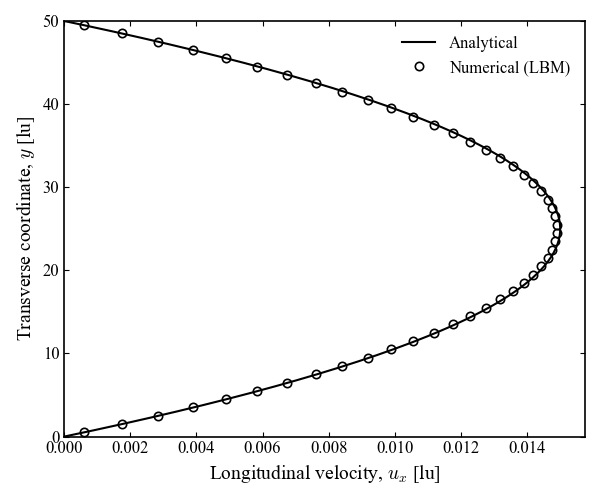
\includegraphics[width=0.5\linewidth]{figuras/validacao_lbm/poiseuille_validacao.png}
    \caption{Numerical longitudinal velocity profile from the LBM solver compared against the analytical Poiseuille parabolic profile at the fully developed cross-section $x = 190$.}
    \label{fig:poiseuille_validation}
\end{figure}

The quantitative convergence analysis validates the incompressibility assumption and the robustness of the boundary schemes.
For the prescribed inlet velocity, the measured mean velocity in the evaluation section was $0.009942$ lu.
The local divergence between the simulated and exact fields resulted in a relative $L_2$ norm error of $6.0272 \times 10^{-3}$.
Furthermore, the absolute deviations remained strictly bounded, yielding a Mean Absolute Error (MAE) of $5.9861 \times 10^{-5}$ lu and a Root Mean Square Error (RMSE) of $6.6025 \times 10^{-5}$ lu, confirming the second-order spatial accuracy characteristic of the standard D2Q9 LBM solver.

\section{Darcy-Brinkman Regime and Permeability Validation}

Having derived the Guo-augmented forcing scheme together with the closed-form drag inversion in Section~\ref{sec:darcy-drag-patch}, and having proved its consistency with the macroscopic Darcy--Brinkman--Navier--Stokes balance via the Chapman--Enskog multiscale expansion of Section~\ref{sec:chapman-enskog}, this section performs the corresponding \emph{numerical} validation of the porous-media branch of the kernel.
The objective is twofold: (i) to verify that, for an imposed intrinsic permeability $K_0$, the LBM solver recovers a numerical permeability $K_{\mathrm{num}}$ within an acceptable tolerance across a sweep of porous regimes, and (ii) to confirm that the simulated transverse velocity profile reproduces the analytical Brinkman solution for the reference case.
Successful execution of both checks demonstrates that the discrete kernel correctly enforces the linear Darcy resistance in the bulk and the Brinkman viscous-shear correction in the boundary layer, validating the porous-media branch of the macroscopic system recovered in equation~\eqref{eq:ce-final-mom}.

\subsection{Data Extraction and $K$ Recovery Methodology}
The numerical validation of the porous resistance was conducted in a $200 \times 50$ lattice domain.
The flow was driven by a constant kinematic inlet ($U_{in} = 0.01$ lu) and constrained by a strict thermodynamic Dirichlet boundary at the outlet ($\rho_{out} = 1.0$).
The complete simulation configuration --- including the \texttt{casos.json} parameter set (\texttt{mode\_m = 0}, $K_0$ sweep), the modified main loop, and the post-processing routine \texttt{validate\_darcy\_flow} that produces the parity and error plots reported below --- is available in the repository branch \texttt{Versao3-Teste-Darcy}\footnote{\url{https://github.com/BorgesMath/LatticeBoltzman/tree/Versao3-Teste-Darcy}}.
To rigorously evaluate the permeability recovery, it is mandatory to eliminate spurious kinetic artifacts generated by non-equilibrium population reconstructions at the open boundaries.
Therefore, the hydrodynamic variables were extracted exclusively from the channel centerline ($y = N_y/2$) within a spatially truncated, fully developed ``bulk region'' defined between $x = 0.25N_x$ and $x = 0.75N_x$.
The thermodynamic pressure $P$ was computed directly from the local density via the LBM isothermal equation of state ($P = c_s^2 \rho$).
For a homogeneous porous medium, Darcy's Law dictates that the longitudinal pressure profile must exhibit a strictly linear drop.
The macroscopic pressure gradient $\nabla P$ was extracted numerically via a linear least-squares regression applied to the centerline pressure nodes within the bulk region.
Subsequently, the algorithm's recovered numerical permeability ($K_{num}$) was calculated by inverting Darcy's equation:
\begin{equation}
    K_{num} = \frac{\nu \bar{\rho} \bar{u}_x}{-\nabla P}
\end{equation}
where $\bar{\rho}$ and $\bar{u}_x$ are the spatially averaged density and longitudinal velocity across the bulk region.

\subsection{Validation Results}
The numerical framework was evaluated against analytical solutions for Brinkman flow in a channel bounded by parallel no-slip walls \cite{brinkman1949calculation}:
\begin{equation}
    u_x(y) = U_{darcy} \left[ 1 - \frac{\cosh\left(\frac{y - H/2}{\sqrt{K_0}}\right)}{\cosh\left(\frac{H}{2\sqrt{K_0}}\right)} \right] \quad \text{where} \quad U_{darcy} = -\frac{\nabla P \cdot K_0}{\nu \bar{\rho}}
\end{equation}

As depicted in Figure~\ref{fig:darcy_profile}, for a baseline test with imposed permeability $K_0 = 10.0$ lu, the LBM solver accurately captured the linear thermodynamic pressure decay (yielding a recovered $K_{num} \approx 9.99$ lu).
The extracted transverse velocity profile perfectly reproduced the analytical plug-flow characteristic induced by the Brinkman viscous resistance.

\begin{figure}[h!]
    \centering
    \framebox{\parbox{0.9\textwidth}{\centering
      \vspace{3cm}
      \textbf{[INSERT: Escoamento de Darcy para validacao.png]} \\
      \small\textit{Left: Linear pressure drop within the bulk region. Right: Transverse velocity profile vs.\ Brinkman analytical solution.}
      \vspace{3cm}
    }}
    \caption{Hydrodynamic validation of the internal resistance field for $K_0 = 10.0$ lu.}
    \label{fig:darcy_profile}
\end{figure}

To map the stability limits of the forcing scheme, an automated parametric sweep was conducted for $K_0 \in [0.5, 20.0]$ lu.
Figure~\ref{fig:darcy_error} confirms an ideal parity between the imposed $K_0$ and the numerical $K_{num}$.

\begin{figure}[h!]
    \centering
    \framebox{\parbox{0.9\textwidth}{\centering
      \vspace{3cm}
      \textbf{[INSERT: Escoamento de Darcy para validacao - Recuperacao de K.png]} \\
      \small\textit{Left: Parity plot ($K_0$ vs.\ $K_{num}$). Right: Relative error distribution.}
      \vspace{3cm}
    }}
    \caption{Permeability recovery performance and relative computational error across different porous regimes.}
    \label{fig:darcy_error}
\end{figure}

The relative computational error remained strictly bounded below $0.8\%$ for all scenarios.
Accuracy maximizes (error $\approx 0.1\%$) at lower permeabilities, where the solid matrix drag dominates viscous diffusion.
This fully validates the thermodynamic consistency of the LBM implementation and the spatial accuracy of the Guo forcing formulation.